\chapter{Di-$b$-jet Search: Outline and Event Selection}
\label{sec:evt}

In Chapter~\ref{sec:theo} it was shown that many Beyond Standard Model theories
predict new particles decaying to one or two $b$-quarks that could be produced by the LHC.
Chapters~\ref{sec:det},~\ref{sec:obj}~and~\ref{sec:trig}
described the detectors and reconstruction techniques used to observe such events in the ATLAS detector.
Hence the motivation and tools required to perform a  search
for resonances decaying to one or two $b$-jets has been outlined.
Such analyses are known as di-$b$-jet searches.

Chapters~\ref{sec:evt},~\ref{sec:bkg}~and~\ref{sec:lim} present two di-$b$-jet searches performed
at the ATLAS detector using a high-mass data-set and a low-mass data-set.
As the analysis structure for the both di-$b$-jet searches is similar the analyses are presented together.

%\vspace{-1em}
\section{Analysis Outline}
\label{sec:evt-outline}

The strategy used for di-$b$-jet searches
can be split up into three parts,
which form the three di-$b$-jet search chapters.
A brief outline of the parts is given here,
and full detail can be found in the relevant chapter.

\begin{itemize}[leftmargin=*]
\item\textbf{Di-$b$-jet Event Selection:} (\textit{Chapter~\ref{sec:evt}})\\
  The first step is to select events that are consistent with a resonance decaying to one or two $b$-quarks
  in a way such that the number of background events is minimised.
  Briefly, two high-momentum jets are required and two $b$-tag categories are considered;
  a category in which both jets have been $b$-tagged (2 $b$-tag) and a category where at least one jet has been $b$-tagged ($\geq$1~$b$-tag).
  This chapter will focus on event selection;
  Section~\ref{sec:evt-datasets} will describe the data-sets used,
  Section~\ref{sec:evt-s+b} will describe the signal and backgrounds
  considered when defining the selections
  and Section~\ref{sec:evt-sel} will set out
  the details of the event selection used for both di-$b$-jet searches.  \vspace{0.8em}

  \vfill \newpage
\item\textbf{Search Phase:} (\textit{Chapter~\ref{sec:bkg}})\\
  Once events have been selected the next part of the analysis aims to determine if there
  is evidence of a new particle in the selected events; this step is known as the `search phase'.
  This step uses the dijet mass (\mjj)~spectrum, where dijet mass is the invariant mass of the two highest \pT{} jets
  \footnote{The two highest \pT{} jets are selected before $b$-tagging is applied}.
  %The production of a new particle is dominated by resonant r
  A new particle will appear as a resonance (or `bump') on the smoothly falling background
  dijet mass distribution from QCD dijet production, as illustrated in Figure~\ref{fig:evt-dijet_schem}.
  The background is modelled using a smoothly falling function and a
  model-independent search for resonances is performed using the {\sc BumpHunter} algorithm~\cite{dibjet-bh}.
  Chapter~\ref{sec:bkg} contains a full description of the search phase strategy and the results of the search phase for both di-$b$-jet searches
  %including tests of the fitting functions used and the results of the search phase in the data-sets considered.
 
  \begin{figure}[!hbt]
  \begin{center}
    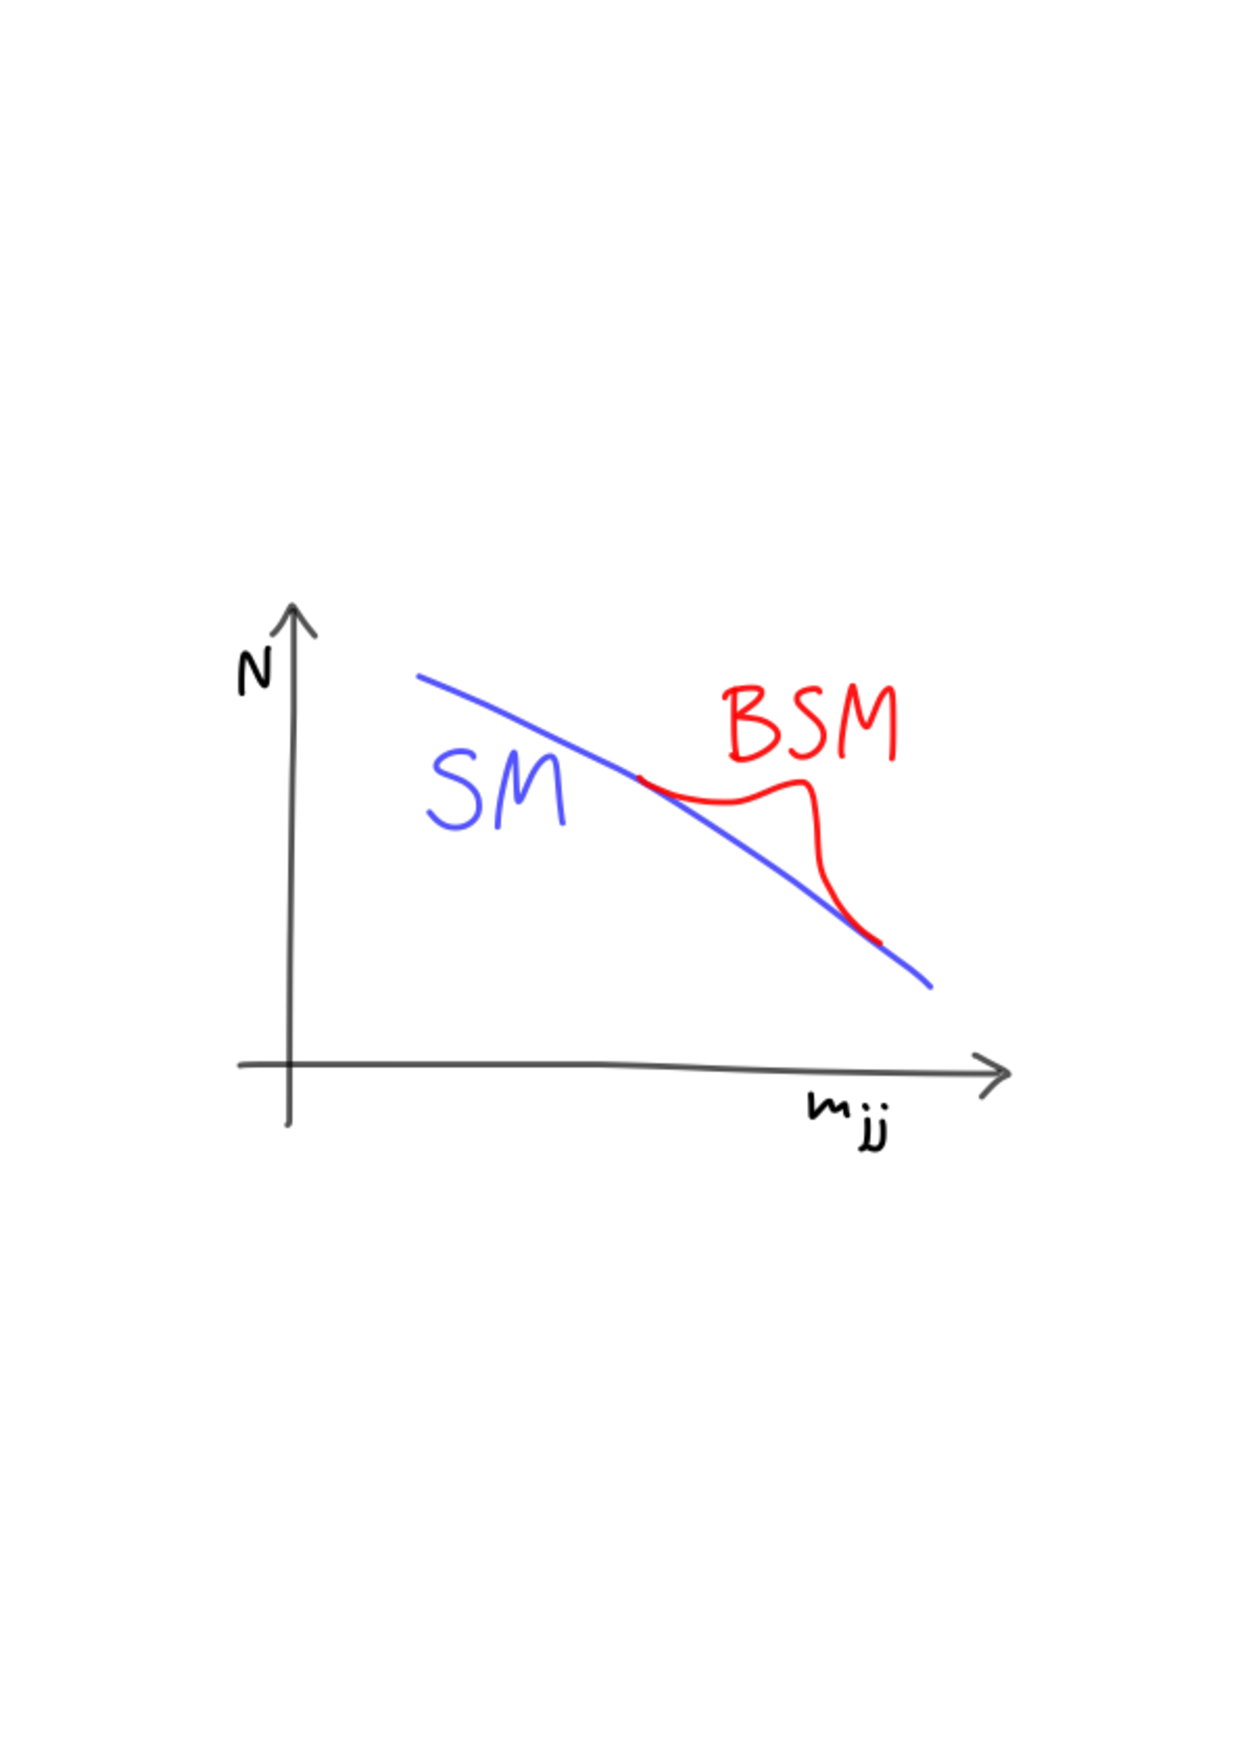
\includegraphics[width=0.6\linewidth, angle=0]{figs/Dibjet/Gen/dijet_schem.pdf}
  \end{center}
  \vspace{-3mm}
  \caption[A cartoon illustrating the use of the dijet mass distribution in the search phase of a di-$b$-jet search.]
          {A cartoon illustrating the use of the dijet mass (\mjj) distribution in the search phase of a di-$b$-jet search.
            Shown is the smoothly falling distribution from QCD dijet production (SM)
            and a resonance shape caused by a Beyond Standard Model (BSM) particle.}
          \label{fig:evt-dijet_schem}
  \end{figure}
  \vspace{-2mm}
 
\item\textbf{Limit Setting:} (\textit{Chapter~\ref{sec:lim}})\\
  If, in the search phase of the analysis, no significant evidence of a resonance is found
  then 95\% confidence level limits are set on the cross-section of the benchmark signal models as a function of mass.
  Chapter~\ref{sec:lim} presents the limit setting methodology,
  a description of the systematic uncertainties and the limit setting results for both di-$b$-jet searches.

\end{itemize}

\section{List of Data Sets Used}
\label{sec:evt-datasets}

Di-$b$-jet searches are performed in several iterations
as data is being collected, where each iteration uses a different data-set.
This is done for two reasons;
firstly it is important to know as soon as possible
if there is evidence of a new resonance as
this would affect the strategy of future di-$b$-jet searches and that of other analyses at ATLAS.
Secondly, this allows us to incrementally
expand, adapt and improve the analysis in each iteration.

In this thesis two different data-sets are considered;
one for a high-mass di-$b$-jet search and one for a low-mass di-$b$-jet search.
The overall analysis strategy is the same for each data-set so the analyses are described together.
However, there are some significant differences in the details;
as such during the analysis description it will be clearly labelled
which data-set is being referred to.

For any data-set a Good Run List (GRL)
is applied to remove events of low data-quality,
which is typically caused by an element of the detector not operating optimally.
For example, data-taking periods where the inner-most layer of the inner detector,
the IBL, was not operating are removed as
this data-taking period has a lower $b$-tagging performance.
A GRL is applied to all data-sets considered in this analysis.

The data-sets are listed below, the trigger used in each data-set is described.
All quoted luminosities are given after the GRL has been applied.

\begin{itemize}[leftmargin=*]
\item\textbf{\summer{}}: \\
  The \summer{} data-set contains 13 TeV $pp$ collision data collected
  between May 2015 and July 2016 corresponding to an integrated luminosity 13.3~\ifb.
  The trigger used in this data-set is \verb|HLT_j380|,
  which requires an online \footnote{Online refers to
    reconstructed objects used in the trigger decision
  whilst offline refers to objects reconstructed after events have passed the trigger at the data-processing level,
  from the definition in Section~\ref{sec:trig-bjet_eff}.}  jet with $\pT~>$~380~GeV, 
  and is chosen as it is the lowest unprescaled single jet trigger \footnote{Unprescaled means that the trigger accepts every event passing the trigger selection criteria}.
  Section~\ref{sec:trig-jet} contains further details on single jet triggers.
  The analysis on this data-set has been published as a conference note~\cite{dibjet-ichep_conf}. \\
  
\item\textbf{\lm{}}: \\
  The \lm{} data-set contains 13 TeV $pp$ collision data collected
  between March 2016 and December 2016, corresponding to an integrated luminosity of 24.3~\ifb.
  The trigger used in this data-set is a double $b$-jet trigger 
  which requires two online jets with $\pT >$ 150~GeV and $\pT >$ 50~GeV
  where both online jets have been $b$-tagged at the trigger level.
  Section~\ref{sec:trig-bjet} contains further details of $b$-jet triggers and the particular trigger used in this analysis.
  The \lm{} data-set uses a $b$-jet trigger as the lower \pT{} thresholds allow
  the analysis to probe a lower range of dijet mass.
  This analysis does not combine data collected in 2015 and 2016, as the $b$-jet trigger configurations used in 2015 and 2016 are significantly different.
  The \lm{} data-set uses a $b$-jet trigger aware GRL which additionally
  removes periods of data where the $b$-jet trigger was performing in a sub-optimal way,
  the GRL is described in Section~\ref{sec:trig-grl}.
  As a double $b$-jet trigger is used only the 2 $b$-tag category is considered.
  The analysis on this data-set is to be published soon.
\end{itemize}

\noindent
In addition there is another data-set being analysed that is not described in this thesis.
\vspace{-0.5em}
\begin{itemize}[leftmargin=*]
\item\textbf{\hm{}}:\\
  The \hm{} data-set contains 13 TeV $pp$ collision data collected
  between May 2015 and December 2016, corresponding to an integrated luminosity of 36.1~\ifb.
  A single jet trigger is used.
  The analysis on this data-set is to be published together with the \lm{} data-set.
\end{itemize}
\vspace{-1em}

\section{Backgrounds and Signal}
\label{sec:evt-s+b}

In the di-$b$-jet event selection two
benchmark signal models and one dominant background are considered.
The signal models and dominant background are
used to optimise event selection.

Monte-Carlo simulations of the background and the signal processes are produced.
Unless specified, all Monte-Carlo simulations are produced using
the \textsc{Pythia8}~\cite{dibjet-pythia8} program for event generation,
the \textsc{EvtGen} package~\cite{trig-evtGen} to model the decays of the $b$ and $c$ hadrons,
and the A14 parameter set~\cite{dibjet-a14} to model the parton shower, hadronisation and underlying event.
The NNPDF23LO PDF set~\cite{dibjet-nnpdf} is used to describe the Parton Distribution Function (PDF) and
the detector response is modelled using the ATLAS detector simulation package~\cite{dijet-sim_ATLAS}.
%The effect of pile-up is modelled by superimposing simulated minimum-bias events
%on the hard-scatter simulation,
%where minimum-bias events are events collected with a loose trigger requirement
%and are dominated by inelastic scattering.

\begin{itemize}[leftmargin=*]
\item\textbf{Background: QCD Di-jet}:  \\
  Section~\ref{sec:theo-qcd} discussed the details of QCD dijet production.
  In particular in Section~\ref{sec:theo-qcd-dijet_features} it was noted that the
  relative strength of the strong force compared to other forces
  of the Standard Model means that QCD dijet production dominates all other backgrounds in a di-$b$-jet event selection.
  %Hence, this will be considered as the only background.
  A description of how the QCD dijet background is modelled in this analysis is described in Chapter~\ref{sec:bkg}.
  A simulated QCD dijet sample is also used in this analysis
  for background studies and background modelling validation.
  \end{itemize}

\noindent
Before describing the signal models used it is useful to clearly differentiate between the two definitions of mass used in this analysis.
The \textit{`dijet mass'} is the invariant mass of the two leading jets, and is denoted by~\mjj.
The \textit{`generated mass'} is defined as the pole mass of the signal model used in the generator.
The two differ due to uncertainties in jet energy measurements.

\begin{itemize}[leftmargin=*]
\item\textbf{Signal: $Z'$ Boson}:  \\
  The $Z'$ boson is an additional gauge boson that can decay to two $b$-quarks.
  The $Z'$ boson models considered are
  described in detail in Section~\ref{sec:theo-bsm_zprime}.
  The $Z'$ boson provides a benchmark model in the 2 $b$-tag category. \vspace{1em}
  %in the case that both jets have been $b$-tagged.

  In the \summer{} and \lm{} data-set analyses
  the Sequential Standard Model (SSM) $Z'$ and the leptophobic $Z'$ models are considered.
  The intrinsic width of the $Z'$ boson has been set to 3\% of the generated mass.
  Monte-Carlo simulation is used to produce dijet mass signal templates at leading order (LO).
  Only decays to $b\bar{b}$ are simulated;
  other decays of the  $Z'$ boson are ignored such that the
  results are easier to interpret for other signal models decaying to pairs of $b$-quarks.
  It has been shown that for a $Z'$ boson model the cross-sections can increase by up to 30\%
  from the addition of next-to-leading order (NLO) diagrams~\cite{evt-NLO_zprime}.
  Therefore the signal template normalisation is corrected to account for NLO effects,
  the correction factors have been derived by comparing
  the LO and NLO matrix calculations performed using the \textsc{MadGraph} generator~\cite{dibjet-madGraph}
  and are found to be between 1.2 and 1.3 depending on the generated mass.
  Simulated SSM and leptophobic $Z'$ boson templates are produced at generated mass points of
  600, 800, 1000, 1250, 1500, 1750, 2000, 2500, 3000, 4000 and 5000~GeV.  \vspace{1em}
  
  Further to this, for the \lm{} data-set
  the Dark Matter inspired (DM) $Z'$ boson is also considered.
  For this model the DM $Z'$ boson signal generation is performed at next-to-leading order using the \textsc{MadGraph5\_aMC@NLO} generator~\cite{dibjet-madGraph_NLO},
  whilst all other aspects of event modelling, including parton shower and hadronisation, are performed using the configuration with \textsc{Pythia8} as described above.
  The coupling of the DM $Z'$ boson to the dark matter fermion ($g_{\chi}$) is set to 1 and
  the mass of the dark matter fermion ($m_{\chi}$) is set to 10 TeV,
  the large value of $m_\chi$ means that decays of the $Z'$ boson to the dark matter fermion are suppressed.
  The coupling to quarks ($g_{SM}$) is set to 0.1,
  decays to $b$, $c$ and light flavour quarks are considered,
  and the generated mass points are 600, 800 and 1000~GeV.
  This configuration is chosen to be consistent with recommendations in~\cite{theo_bsm-zprime_dm}
  and to be consistent with other dijet searches at ATLAS~\cite{dijet-mori16_paper}.  \vspace{1em}
  %Similarly the same models are considered in the \lm{}... \\

\item\textbf{Signal: $b^*$ Quark}:   \\ 
  The $b^*$ quark is a third generation excited quark which results from
  quark compositeness models.
  The dominant decay mode of the  $b^*$ quark is to $bg$.
  The model considered is
  described in detail in Section~\ref{sec:theo-bsm_bstar}.
  The $b^*$ quark provides a benchmark model in the $\geq$1~$b$-tag category.  \vspace{1em}
  %case that at least one of the jets has been $b$-tagged.
  
  For the \summer{} data-set the same $b^*$ quark model is considered.
  Monte-Carlo simulation is used to produce a $b^*$ quark dijet mass signal template.
  Only leading order calculations are considered.
  %again \textsc{Pythia8}~\cite{dibjet-pythia8} with the A14~\cite{dibjet-a14} tune and the NNPDF23LO PDF set~\cite{dibjet-nnpdf} is used.
  Decays to $bg$, $b\gamma$, $bZ_0$ and $tW^{-}$ are considered
  \footnote{Using the branching ratios described in Section~\ref{sec:theo-bsm_bstar}.}.
  %further details can be found in Section~\ref{sec:evt-sel-btag}.
  Simulated $b^*$ quark signal templates are produced at generated mass points of
  1250, 1500, 1750, 2000, 2500, 3000, 4000 and 5000~GeV.
  In the \lm{} data-set the $b^*$ quark model is not considered 
  as only the 2 $b$-tag category is used.
\end{itemize}

\section{Event Selection}
\label{sec:evt-sel}

The overall aim when designing the di-$b$-jet event selection
is two-fold.
Firstly, events are selected to
maximise sensitivity to signal;
which is approximated in terms of $S$/$\sqrt{B}$,
where $S$ is the number of benchmark signal events and $B$ is the number of background events.
Secondly, the smoothly falling nature of the background needs to be maintained
as this is the underlying assumption of the background estimation strategy,
which will be described in Chapter~\ref{sec:bkg}.
Here, smooth means that the spectrum is monotonically decreasing with no discontinuities.
%In addition, it is desirable that the event selection for the
%\hm{} and \lm{} data-set are
%harmonised where possible as the two analyses are to be published together.
%Any differences in event selection between the two must be well motivated.

The di-$b$-jet event selection is split up into three parts, with each part described in a separate section.
Firstly, a pair of jets are selected (Section~\ref{sec:evt-sel-jets}),
then a set of event-level kinematic cuts are applied using the selected jets (Section~\ref{sec:evt-sel-event})
and finally $b$-tagging is applied to the jets (Section~\ref{sec:evt-sel-btag}).
In Section~\ref{sec:evt-sel-acc} the full event selection is summarised and
the signal acceptance is evaluated.

The event selection is different for the high-mass and low-mass data-sets considered,
these differences will be noted and discussed in the text.

\subsection{Jet Selection}
\label{sec:evt-sel-jets}

Jets are reconstructed using the anti-$k_T$ algorithm~\cite{obj-jets_reco_akt} with $R=0.4$
and calibrated using the EM+JES scheme;
a full description of jets used in this analysis is in Section~\ref{sec:obj-jets}.

At least two jets are required in an event.
The two highest \pT{} jets, referred to as the leading and subleading jet,
are the jets used throughout this analysis.
To reduce the number of fake jets from sources such as calorimeter noise
both jets are required to pass \textit{loose} jet cleaning cuts
based on the properties and distributions of the energy deposits in the calorimeter associated to the jet;
details can be found in~\cite{evt-jet_cleaning}.

Requirements are placed on  the leading and subleading jet-\pT{} such that events are on the trigger plateau;
the kinematic region where all events that pass the offline jet-\pT{} requirements
also pass the online jet-\pT{} requirements of the trigger.
To be on the trigger plateau of a single jet trigger the offline jet-\pT{} must be above some threshold value,
which is referred to as the threshold jet-\pT{}.

For the \summer{} data-set; it is required that the leading jet has \pT{}~$>$~430~GeV to be on the trigger plateau of \verb|HLT_j380|.
This cut is derived by comparing the leading jet-\pT{} distributions of jets that pass the trigger, \verb|HLT_j380|,
relative to a reference trigger with a lower jet-\pT{} threshold, \verb|L1_J75|.
Figure~\ref{fig:evt-ICHEP_turnon}(a) shows the leading jet-\pT{}
of events that pass the single jet triggers \verb|HLT_j360| (red), \verb|HLT_j380| (green) and \verb|HLT_j400| (blue)
compared to events that pass the reference trigger \verb|L1_J75| (black),
in one run of data where \verb|L1_J75| is unprescaled.
In the ratio it is shown that for leading jet-\pT{}~$>$~430~GeV events are on the trigger plateau of \verb|HLT_j380|.
The subleading jet is required to have jet-\pT{}~$>$~60~GeV
to reduce contamination from pile-up jets
\footnote{Specifically, if jets have \pT{} $<$ 60~GeV then it is recommended that
  a pile-up suppression algorithm known as Jet Vertex Tagger (JVT) is used~\cite{evt-jvt}.
  There is little gain in acceptance from the addition of low \pT{} subleading jets and
  complications from implementing the recommendations so the jets are removed. }.
Both jets  are required to have $|\eta| <$ 2.4
such that the jets lie within the volume of the ATLAS pixel detector,
which is essential for optimal $b$-tagging performance.

\begin{figure}[!ht]
  \begin{center}
    \captionsetup[subfigure]{aboveskip=0pt,justification=centering}
    \hspace{-2mm}
    \subcaptionbox{Leading Jet-\pT{}} {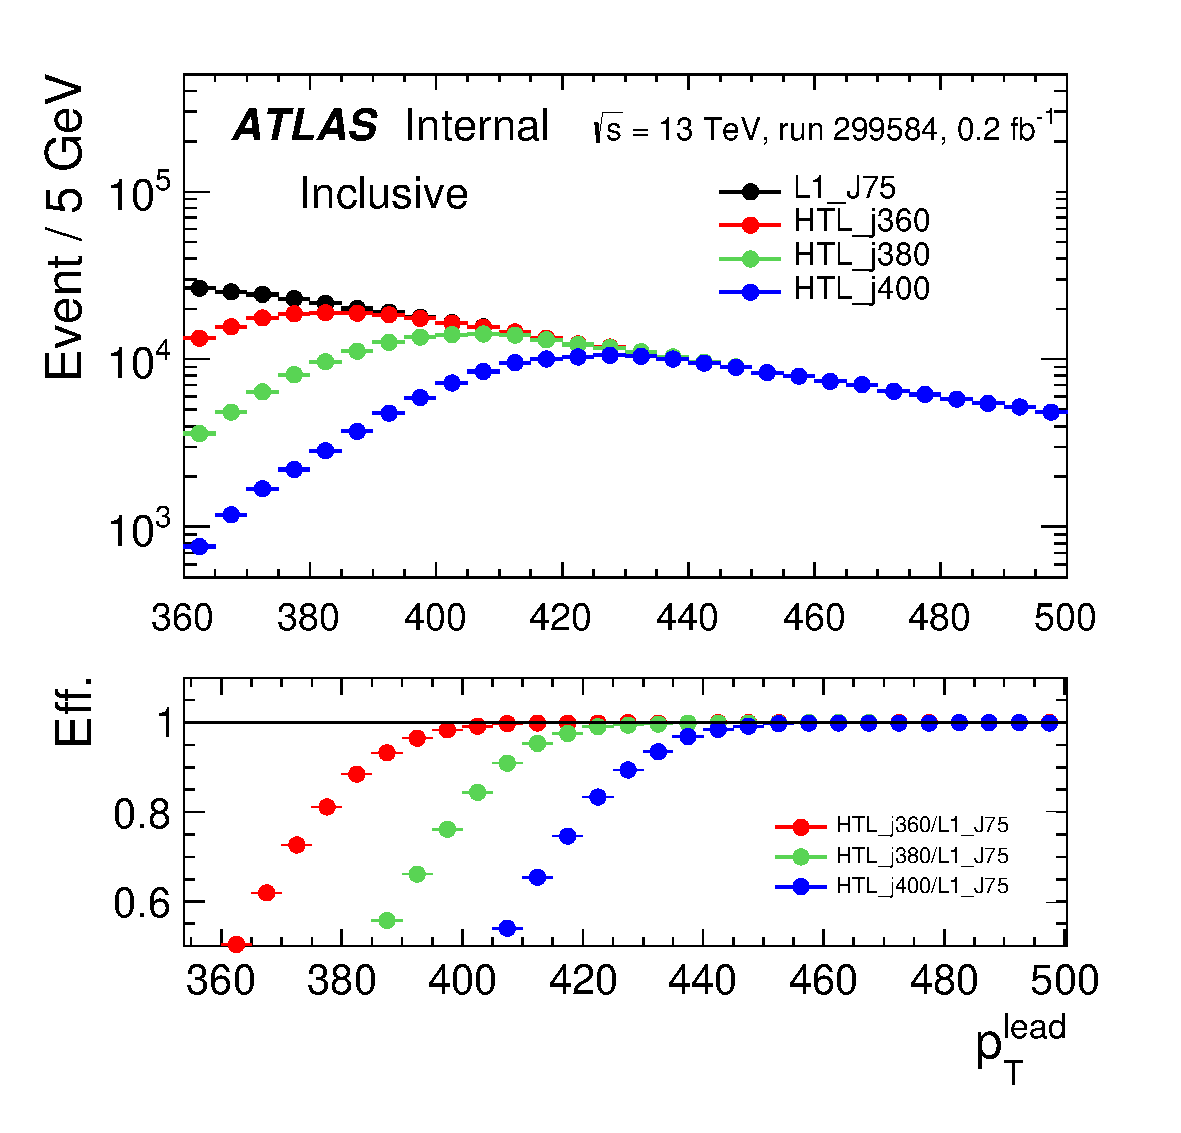
\includegraphics[width=0.47\linewidth, angle=0]{figs/Dibjet/ICHEP/evt-jet_pt.pdf}}
    \subcaptionbox{\mjj}              {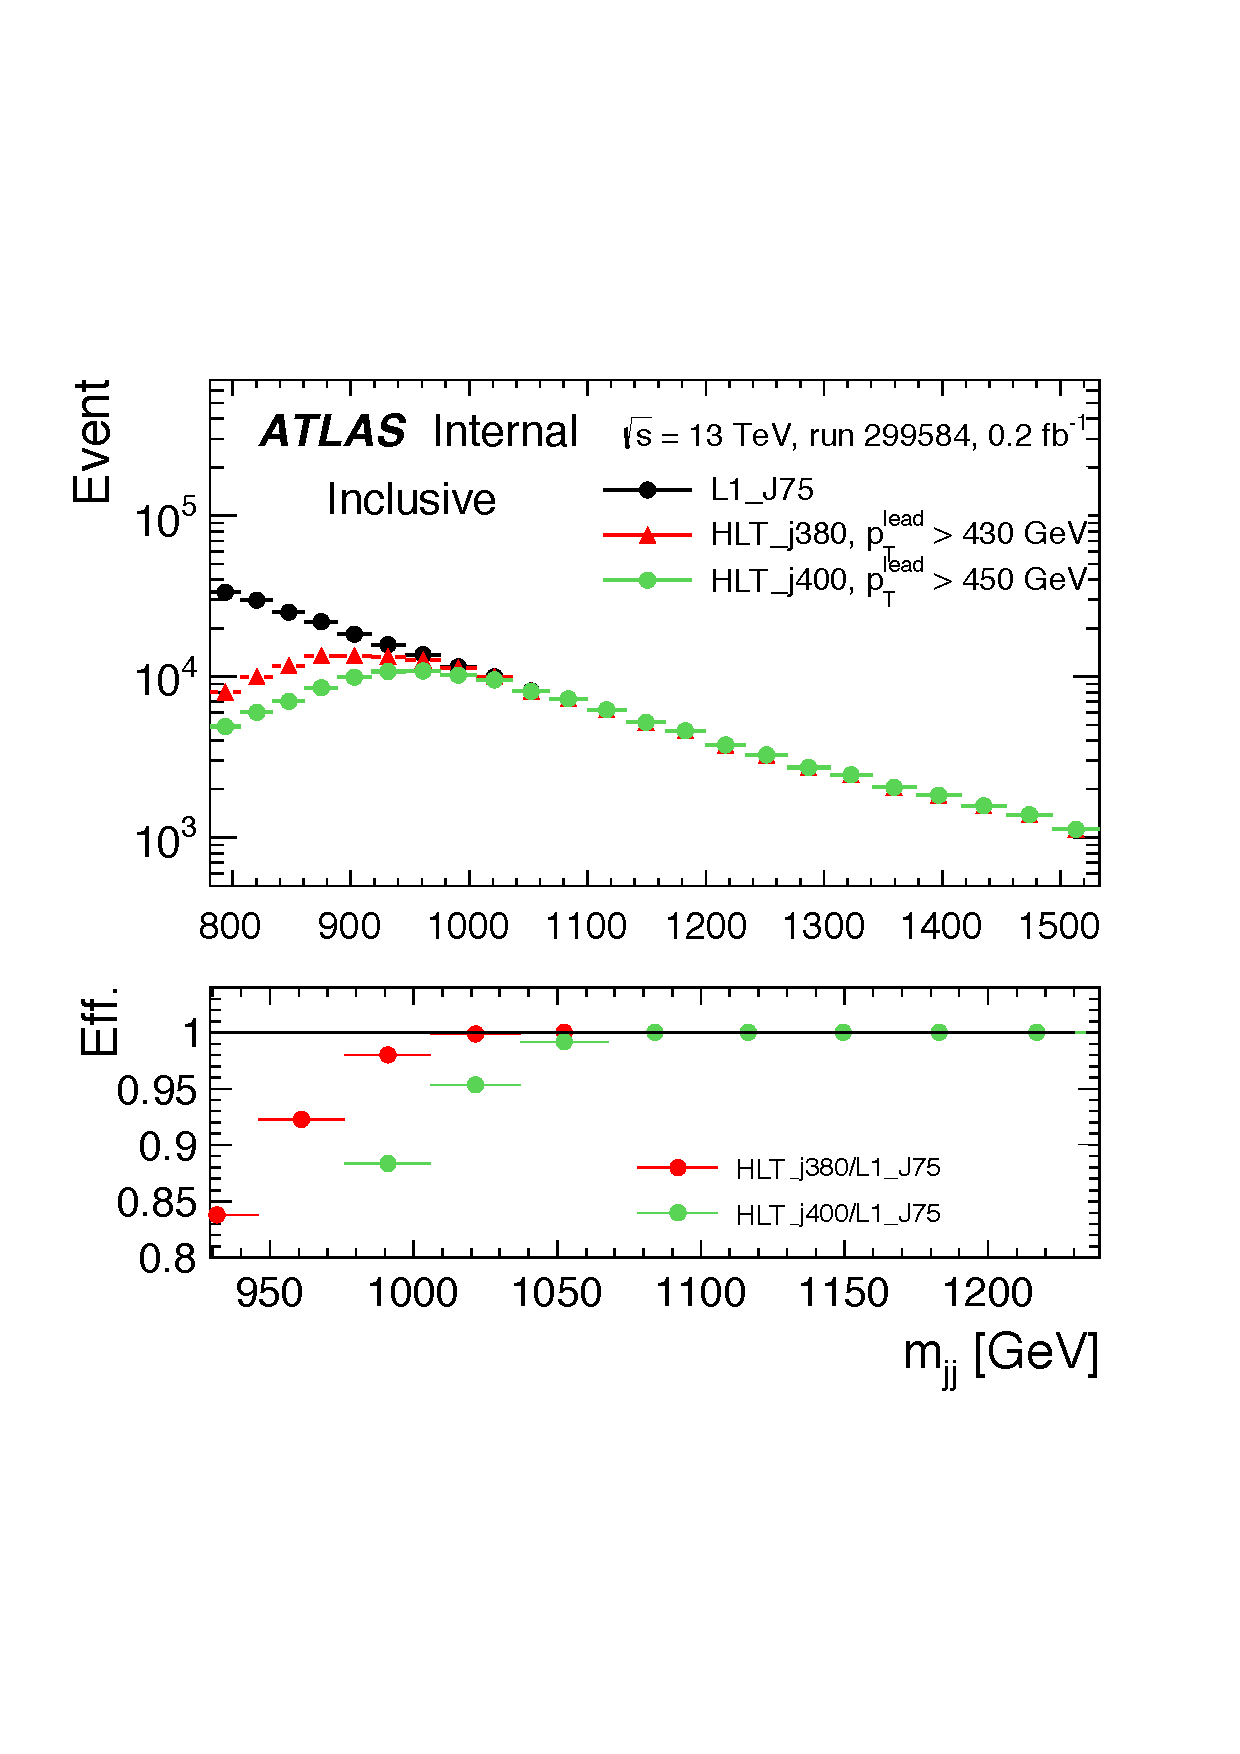
\includegraphics[width=0.46\linewidth, angle=0]{figs/Dibjet/ICHEP/evt-mjj.pdf}}
  \end{center}
  \vspace{-1em}
  \caption[Derivations of the leading jet-\pT{} and \mjj{} cuts for the \summer{} data-set event selection using events that pass an
            unprescaled L1\_J75 trigger compared to events that pass a range of single-jet triggers in one run of 2016 data.]
          {The comparisons of the (a) leading jet-\pT{} ($\pT^{\text{lead}}$) and (b) dijet mass (\mjj{})~using events that passed an
            unprescaled L1\_J75 trigger (black) compared to events that pass a range of single-jet triggers (coloured) in one run of 2016 data.
            As shown in the legend, the single-jet triggers considered are HLT\_j380, HLT\_j400 and, in plot (a), HLT\_j360.
            In plot (b) the \summer{} event selection (excluding $b$-tagging) is applied with a leading jet-\pT{} cut as described in the legend.
            The ratio with respect to L1\_J75 is shown in the lower panel~\cite{dibjet-ichep_conf}.}
     \label{fig:evt-ICHEP_turnon}
\end{figure}

%For the \hm{} data-set the trigger \verb|HLT_j380| is also used,
%and as such the leading jet is again required to have \pT{}~$>$~430~GeV.
%The subleading jet is required to have \pT{}~$>$~80~GeV to be consistent with the subleading jet-\pT{} requirement of the \lm{} event selection,
%which will be described in the following paragraph.
%Both jets  are required to have $|\eta| <$ 2.0;
%the tighter cut on $|\eta|$ (relative to the \summer{} data-set) is selected as the
%$b$-jet energy scale uncertainty is significantly increased at large values of jet-$|\eta|$.

For the \lm{} data-set a double $b$-jet trigger is used;
which requires that there is one online jet with $\pT~>$~150~GeV and another online jet with $\pT~>$~50~GeV.
Therefore, to be on the trigger plateau the leading jet-\pT{} is required to be above the threshold jet-\pT{}
of a single jet trigger that requires an online jet with $\pT~>$~150~GeV
and the subleading jet-\pT{} is required to be above the threshold jet-\pT{}
of a single jet trigger that requires online jet-$\pT~>$~50~GeV.
To find the threshold jet-\pT{} of the two single-jet triggers,
a linear fit to the threshold jet-\pT{} of a range of single jet triggers is used,
details are in Appendix~\ref{app:triggerTurnOn_fit}.
Using the results of the linear fit the leading jet is required to have \pT{}~$>$~200~GeV
and the subleading jet is required to have \pT{}~$>$~80~GeV.
Both jets  are required to have $|\eta| <$ 2.0;
the tighter cut on $|\eta|$ (relative to the \summer{} data-set) is selected as the
$b$-jet energy scale uncertainty is significantly increased at large values of jet-$|\eta|$.
%Both jets  are required to have $|\eta|~<$~2.0 to be consistent with the \hm{} event selection.

%\begin{figure}[!ht]
%  \begin{center}
%    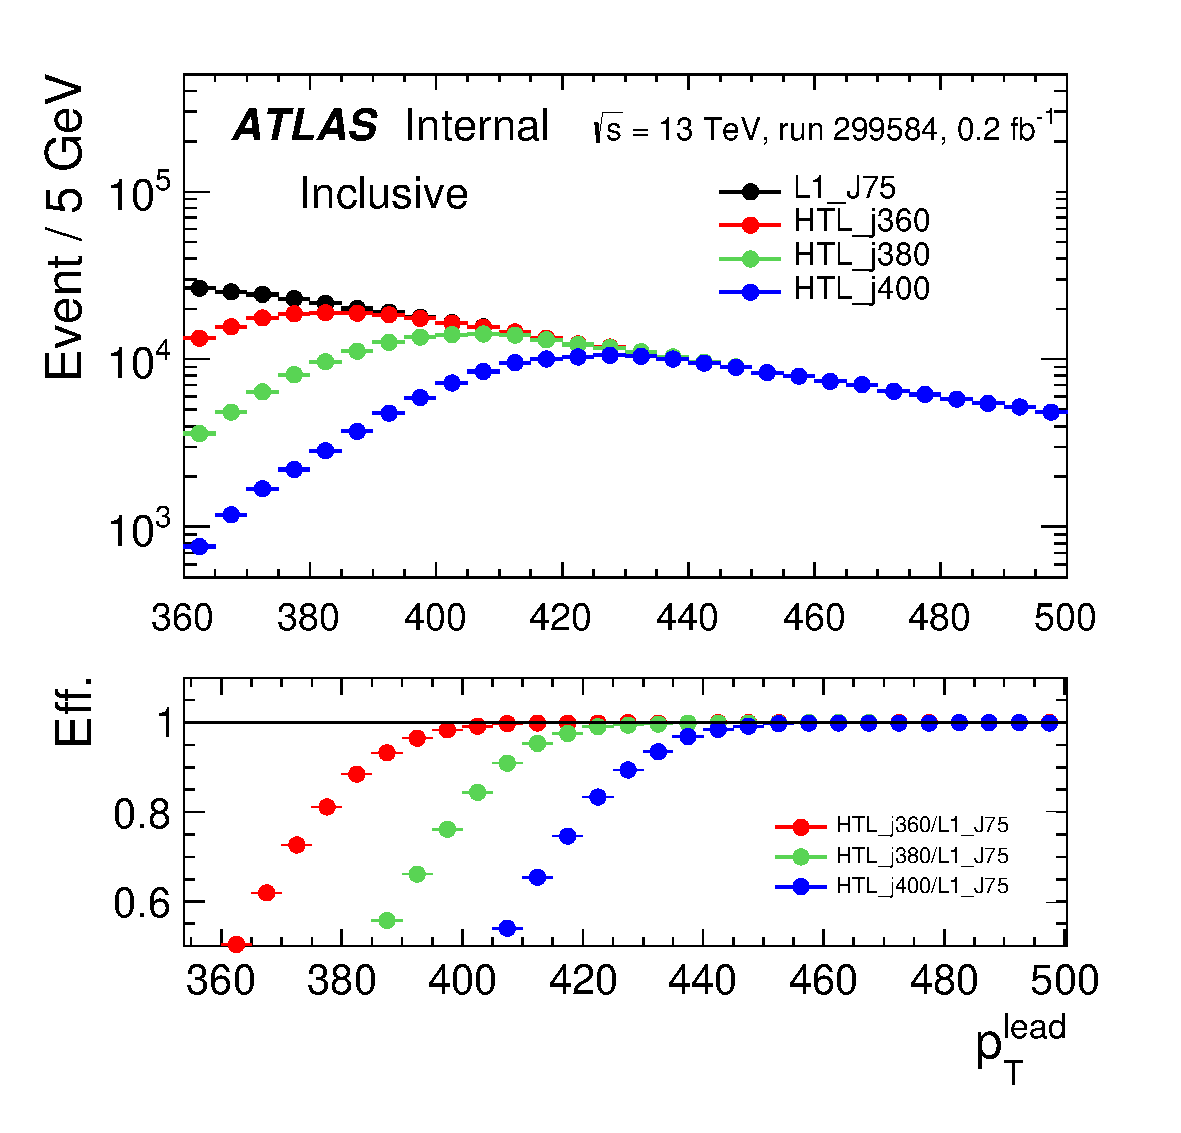
\includegraphics[width=0.8\linewidth, angle=0]{figs/Dibjet/ICHEP/evt-jet_pt.pdf}
%  \end{center}
%  \caption[The comparisons of the leading jet-\pT{} using unprescaled L1\_J75 trigger (black dots) to the HLT\_J360 trigger (red dots),
%    HLT\_J380 trigger (green dots) and HLT\_J400 trigger (blue dots) in one run of 2016 data.
%  The ratio with respect to L1\_J75 is shown in the lower panel.]
%        {The comparisons of the leading jet-\pT{} using an unprescaled L1\_J75 trigger (black dots) to the HLT\_J360 trigger (red dots),
%          HLT\_J380 trigger (green dots) and HLT\_J400 trigger (blue dots) in one run of 2016 data.
%          The ratio with respect to L1\_J75 is shown in the lower panel~\cite{dibjet-ichep_conf}.}
%  \label{fig:evt-jet_pt}
%\end{figure}

\subsection{Event-Level Cuts}
\label{sec:evt-sel-event}

The next part of the event selection is a set of event-level requirements using the two selected jets.
Firstly, the primary vertex must have at least two  tracks associated with it
to ensure good primary vertex reconstruction,

\noindent
Secondly, there is a cut applied to the variable $y^*$, defined as
\begin{equation}
  y^* = \frac{(y_1-y_2)}{2}
\end{equation}
where $y_1$ and $y_2$ are the rapidities of the leading and subleading jet respectively.
As discussed in Section~\ref{sec:theo-qcd-dijet_features}, QCD dijet production can occur through $t$-channel processes leading to more background events at large values of $|y^*|$,
whilst signal production occurs only through $s$-channel processes so will have no dependence on $y^*$.
Therefore, requiring that $|y^*|$ is below some threshold value will lead to increased sensitivity.

For both the \summer{} and \lm{} data-sets it is required that $|y^*| <$ 0.6.
This value has been shown to maximise $S/\sqrt{B}$ when no $b$-tagging is applied
in previous inclusive dijet searches at ATLAS~\cite{dijet-mori16_paper}
\footnote{Inclusive dijet analysis means a dijet analysis where no $b$-tagging is applied.},
where $S$ is the number of benchmark signal events and $B$ is the number of background events.
The effect of $b$-tagging on the optimal value of this cut is assumed to be small,
as $t$-channel processes still dominate the background.

%In the \hm{} data-set it is required that $|y^*| <$ 0.8.
%This value is found by maximising $S/\sqrt{B}$ in the 2 $b$-tag category for a range of generated mass points
%using the SSM $Z'$ boson model as signal and the QCD background from simulation as background.

%In the \lm{} data-set it is required that $|y^*| <$ 0.6.
%The $|y^*|$ cut was not harmonised with the \hm{} data-set
%as it was shown that the looser cut introduced a kinematic bias at low values of dijet mass.
%This will be demonstrated below.

The dijet mass, \mjj{}, is required to be above a threshold value to ensure that two conditions are met.
Firstly it is required that there is no kinematic bias on the dijet mass distribution
caused by the trigger or jet-\pT{} requirements described in Section~\ref{sec:evt-sel-jets}.
Secondly, it is also required that the background is smooth in the dijet mass region chosen
such that it can be described using our background modelling strategy.

In the \summer{} data-set it is required that \mjj~\gt~1378~GeV;
which ensures the two conditions listed above are met.
Firstly, Figure~\ref{fig:evt-ICHEP_turnon}(b) shows the dijet mass spectra for events
that pass the trigger \verb|HLT_j380| and the \summer{} jet-\pT{} requirements
compared to events that pass a reference trigger, \verb|L1_J75|,
in one run of data where \verb|L1_J75| is unprescaled.
For both spectra events are required to pass the jet-$|\eta|$ and $|y^*|$ requirements of the \summer{} event selection.
The ratio plot demonstrates that for \mjj~\gt~1100~GeV there is no kinematic bias from the trigger or event selection.
Secondly, it has been shown using simulated events that
\mjj~\gt~1378~GeV is required such that the dijet mass distribution from QCD dijet production
can be described by our background modelling strategy;
this study is presented in Section~\ref{sec:bkg-summer_range}.
Hence, \mjj~\gt~1378~GeV is the loosest cut that meets both of the conditions.

%In the \hm{} data-set it is required that \mjj~\gt~1200~GeV in the 2 $b$-tag category and
%\mjj~\gt~1341~GeV in the $\geq1$ $b$-tag category;
%which again ensures the two conditions discussed above are met.
%Firstly, Figure~\ref{fig:evt-hm_turnon} compares the dijet mass spectrum
%for events that pass the trigger \verb|HLT_j380| and the \hm{} jet-\pT{} requirements
%to events that pass a reference trigger, \verb|L1_J75|.
%The comparison is done in one run of data where \verb|L1_J75| is unprescaled.
%For both spectra it is required that events pass the $y^*$ and jet-$\eta$ requirements of the \hm{} event selection.
%The ratio plot demonstrates that for \mjj~\gt~1200~GeV there is no kinematic bias from the trigger or event selection.
%Secondly, it will be shown in Section~\ref{sec:bkg-hm_spsig_1b}
%that in the $\geq1$ $b$-tag category a cut of \mjj~\gt~1341~GeV is required such that the
%dijet mass distribution from the background can be described by our background modelling strategy.
%No such effect was observed in the 2 $b$-tag category.
%Hence, \mjj~\gt~1200~GeV is required in the 2 $b$-tag category and
%\mjj~\gt~1341~GeV is required in the 1 $b$-tag category.

%\begin{figure}[!ht]
%  \begin{center}
%    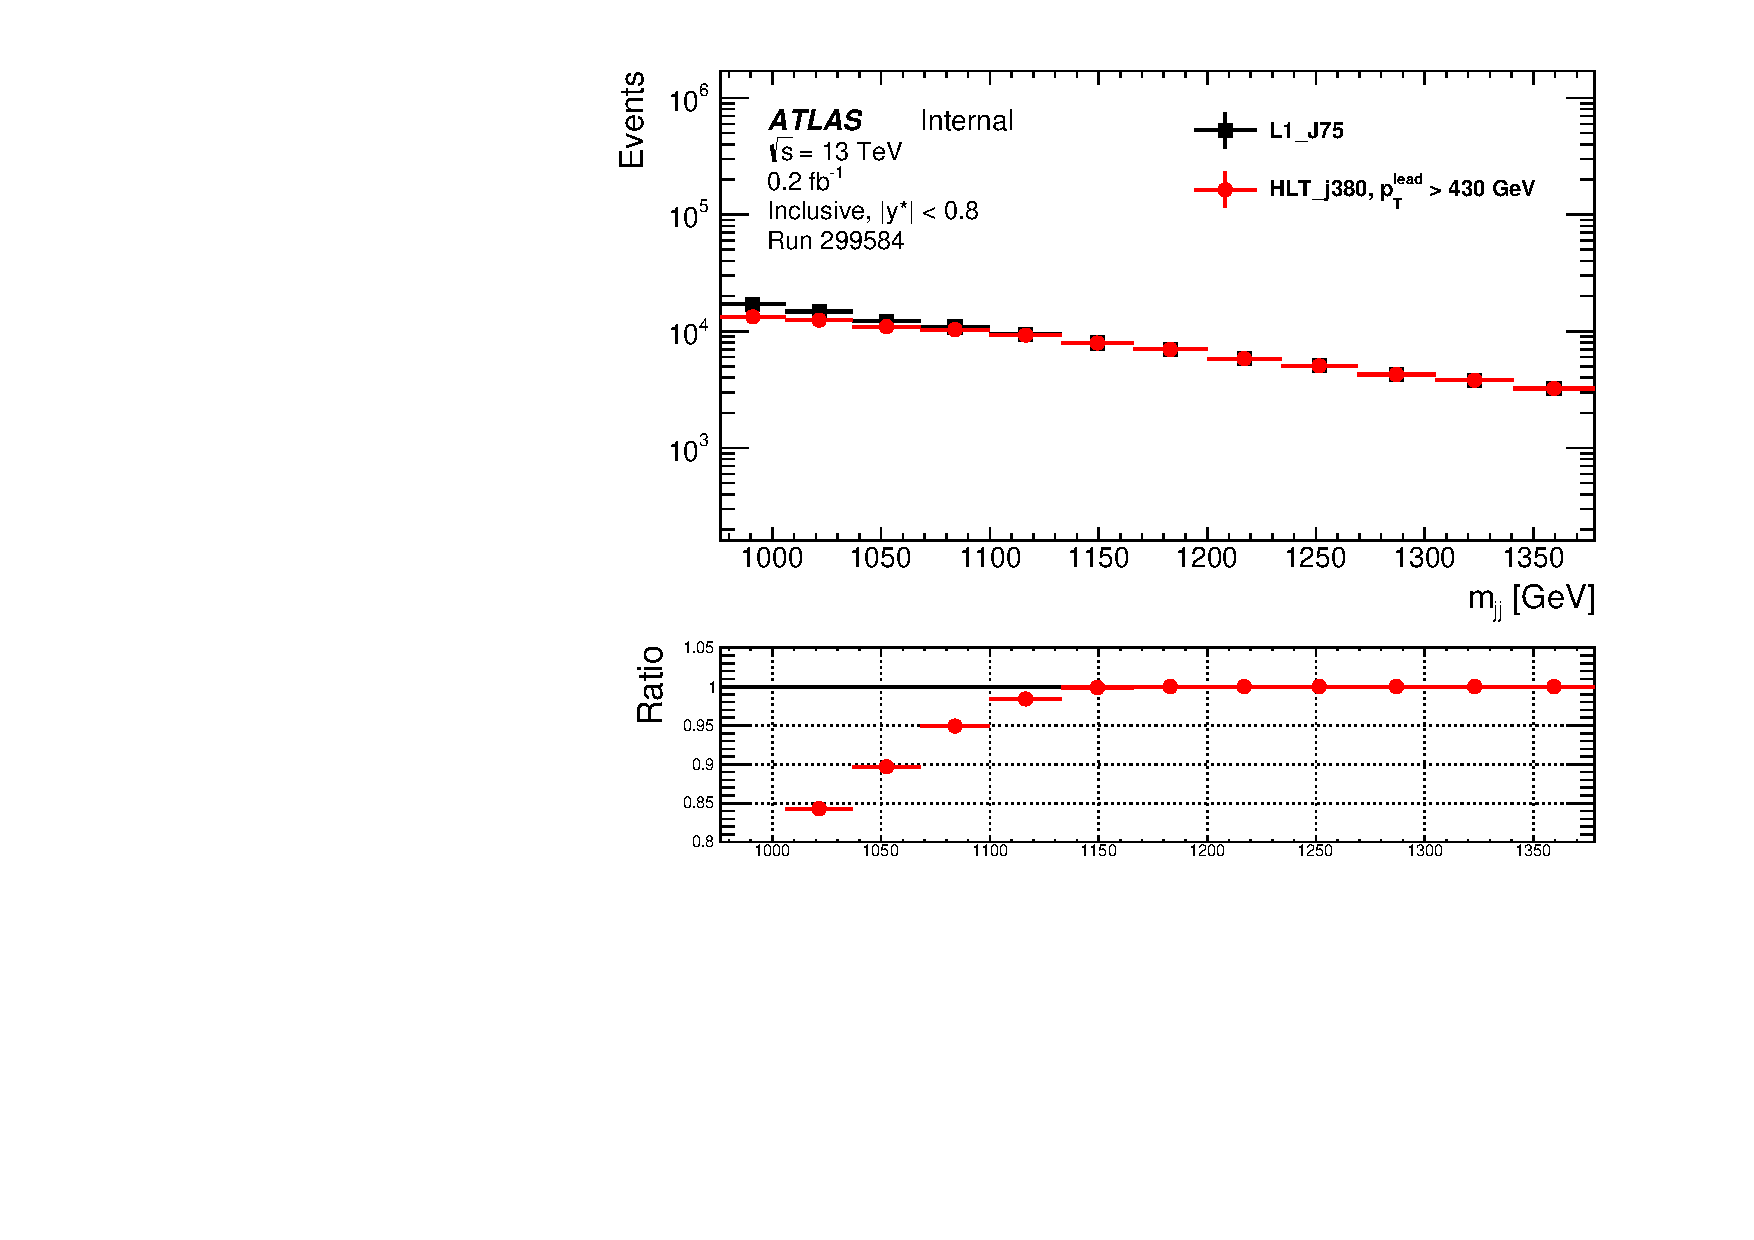
\includegraphics[width=0.6\linewidth, angle=0]{figs/Dibjet/HighMass/evt-mjj.pdf}
%  \end{center}
%  \caption{The comparisons of the dijet mass (\mjj{}) spectrum of events that pass an unprescaled L1\_J75 trigger (black squares)
%    and events that pass the  HLT\_j380 trigger and the \hm{} event selection jet-\pT{} requirements (red dots)
%    in one run of 2016 data where L1\_J75 is unprescaled.
%    The \hm{} event selection requires that leading jet \pT{} ($\pT^{lead}$)~\gt~430~GeV and subleading jet-\pT{} \gt~80~GeV.
%    The jet-$|\eta|$ and $|y^*|$ of the \hm{} event selection have been applied.
%    The ratio with respect to L1\_J75 is shown in the lower panel.}
%     \label{fig:evt-hm_turnon}
%\end{figure}

For the \lm{} data-set it is found that for \mjj~\gt~500~GeV there is no kinematic bias
from the jet-\pT{} cuts used in the \lm{} data-set event selection.
Figure~\ref{fig:evt-lowmass_turnon} compares the dijet mass distribution of events
that pass the event selection requirements that the leading (subleading) jet-\pT{}~$>$~200~(80)~GeV, labelled as `analysis~cuts',
compared to events that pass lower requirements that the leading (subleading) jet-\pT{}~$>$~150~(50)~GeV, labelled as `low~cuts'.
Events are required to pass the \verb|L1_J75| trigger and are taken from a run of 2016 data where \verb|L1_J75| was unprescaled.
The events are additionally required to pass the jet-$|\eta|$ and $|y^*|$ requirements of the \lm{} data-set event selection.
For \mjj~\gt~500~GeV there is no kinematic bias from the \lm{} event selection,
this includes a one dijet mass bin buffer that is used as a safety measure.

%For the \lm{} data-set it is found that for \mjj~\gt~500~GeV there is no kinematic bias
%from the jet-\pT{} cuts used in the \lm{} data-set event selection.
%Figure~\ref{fig:evt-lowmass_turnon}(a) compares the dijet mass distribution of events
%that pass the event selection requirements that the leading (subleading) jet-\pT{}~$>$~200~(80)~GeV, labelled as `analysis~cuts',
%compared to events that pass lower requirements that the leading (subleading) jet-\pT{}~$>$~150~(50)~GeV, labelled as `low~cuts'.
%Events are required to pass the \verb|L1_J75| trigger and are taken from a run of 2016 data where \verb|L1_J75| was unprescaled.
%The events are additionally required to pass the jet-$\eta$ and $|y^*|$ requirements of the \lm{} data-set event selection.
%For \mjj~\gt~500~GeV there is no kinematic bias from the \lm{} event selection,
%this includes a one~\mjj~bin buffer that is used as a safety measure.
%Figure~\ref{fig:evt-lowmass_turnon}(b) shows an identical comparison of  dijet mass distribution
%when it is required that $|y^*|~<$~0.8.
%For $|y^*|~<$~0.8 there is a kinematic bias in the dijet mass range 500-544~GeV,
%and as such the $|y^*|~<$~0.8 is not used in the event selection.


\begin{figure}[!ht]
  \begin{center}
    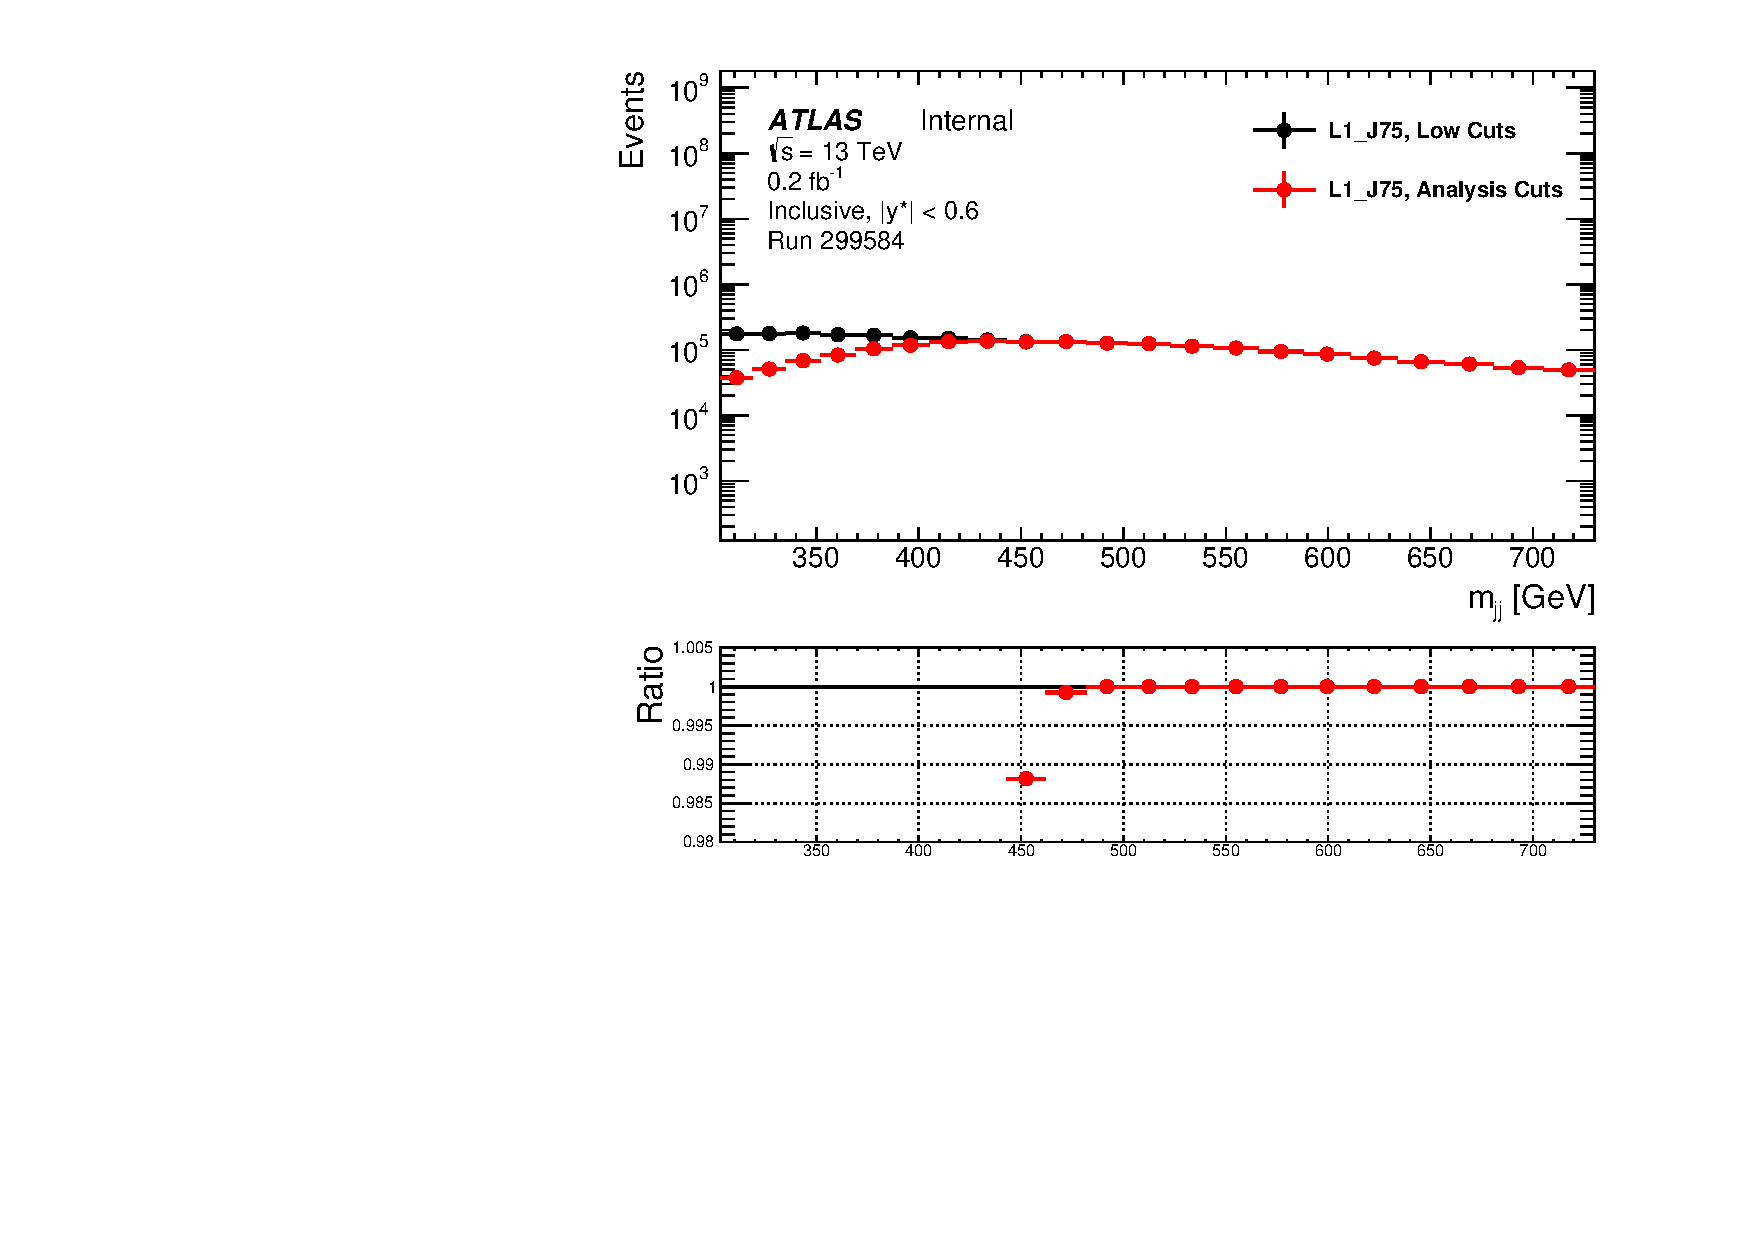
\includegraphics[width=0.55\linewidth, angle=0]{figs/Dibjet/LowMass/evt-mjj_yStar0p6.pdf}
  \end{center}
  \vspace{-1em}
  \caption[Derivations of the dijet mass cut for the \lm{} data-set event selection.]
          {Comparisons of the dijet mass (\mjj{})~of events that pass the analysis jet-\pT{} cuts of leading (subleading) jet-\pT{}~$>$~200 (80)~GeV (red)
    compared to events that pass a set of low jet-\pT{} cuts of leading (subleading) jet-\pT{}~$>$~150 (50)~GeV (black).
    The events are required to pass the L1\_J75 trigger and are taken from one run of 2016 data where the trigger L1\_J75 is unprescaled.
    Events are required to have $|y^*| <$ 0.6 and no $b$-tagging requirements have been applied.}
     \label{fig:evt-lowmass_turnon}
\end{figure}


%\begin{figure}[!ht]
%  \begin{center}
%    \captionsetup[subfigure]{aboveskip=0pt,justification=centering}
%    \subcaptionbox{$|y^*| <$ 0.6} {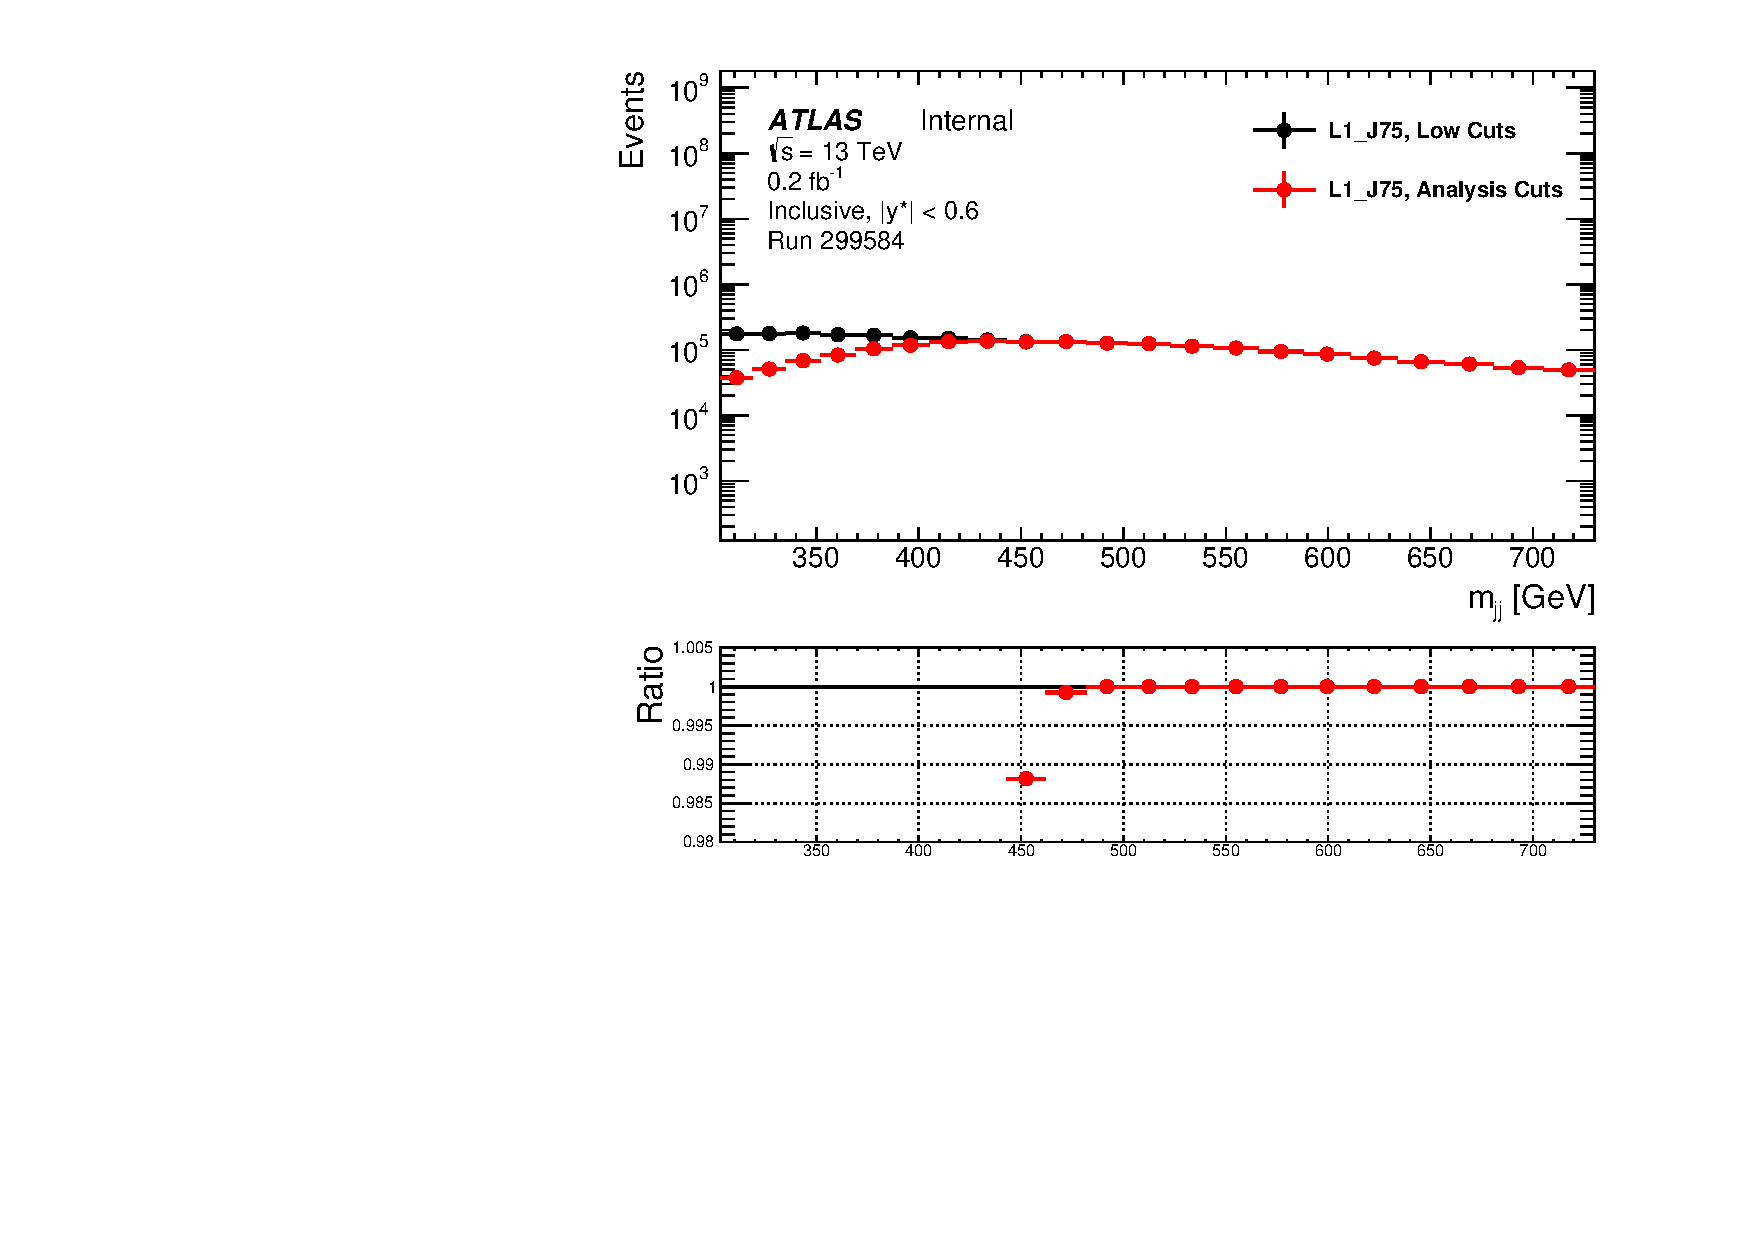
\includegraphics[width=0.5\linewidth, angle=0]{figs/Dibjet/LowMass/evt-mjj_yStar0p6.pdf}}\hspace{-2mm}
%    \subcaptionbox{$|y^*| <$ 0.8} {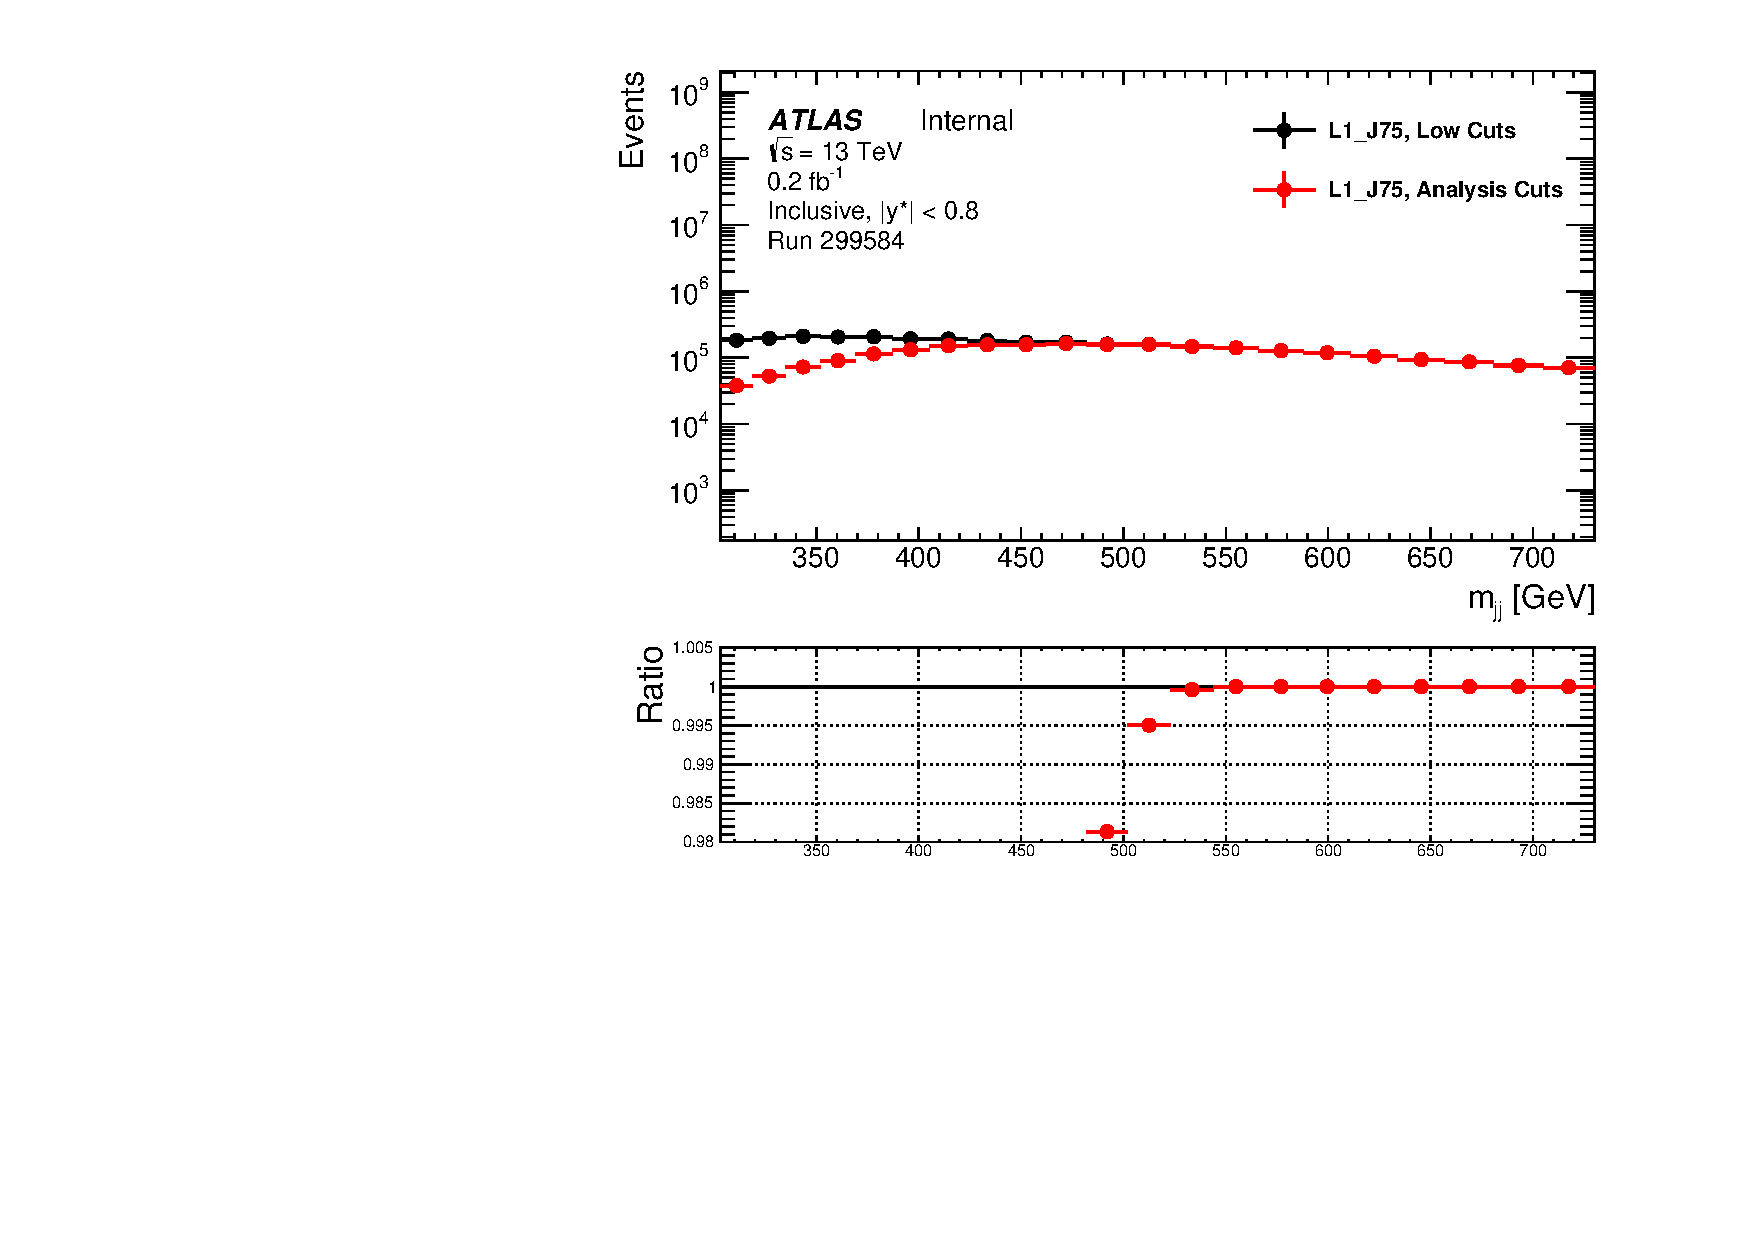
\includegraphics[width=0.5\linewidth, angle=0]{figs/Dibjet/LowMass/evt-mjj_yStar0p8.pdf}}
%  \end{center}
%  \caption{Comparisons of the dijet mass (\mjj{})~of events that pass the analysis jet-\pT{} cuts of leading (subleading) jet-\pT{}~$>$~200 (80)~GeV (black)
%    compared to events that pass a set of low jet-\pT{} cuts of leading (subleading) jet-\pT{}~$>$~200 (80)~GeV (red).
%    The events are required to pass the L1\_J75 trigger and are taken from one run of 2016 data where the trigger L1\_J75 is unprescaled.
%    In addition the events are required to have (a) $|y^*| <$ 0.6 and (b) $|y^*| <$ 0.8.
%    No $b$-tagging cuts have been applied.}
%     \label{fig:evt-lowmass_turnon}
%\end{figure}

However, for the \lm{} data-set
there is an additional kinematic bias on dijet mass 
due to the effect of jets other than the leading or subleading jet
that was discovered as the analysis progressed.
To account for this effect it is required that \mjj{}~\gt{}~566~\GeV{}.
The studies showing this effect are described below in Section~\ref{sec:evt-sel_btrigMatch}
as the $b$-tagging selections used in the \lm{} event selection must be introduced first

For the \lm{} data-set the upper bound of the dijet mass range considered by the search phase is 1533~GeV.
This value is chosen such that there is no gap in the mass range searched by the low-mass and high mass di-$b$-jet searches.
%There is no need for the \lm{} analysis to consider higher masses as in this mass range the \hm{} data-set
%analysis will be more sensitive to signal.% due to the looser $b$-tagging requirements.

\subsection{$b$-Tagging}
\label{sec:evt-sel-btag}

The selection of $b$-jets, known as $b$-tagging,
forms an essential technique in the di-$b$-jet event selection.
A detailed description of $b$-tagging is found in Section~\ref{sec:obj-bjets}.
$b$-Tagging is performed using a multi-variate algorithm known as MV2c10 which has been described in Section~\ref{sec:obj-bjets_MV2}.

Two $b$-tagging categories are used for the two different types of signal model considered.
The 2 $b$-tag category requires that both jets are $b$-tagged,
and is used to search for resonances decaying to 2 $b$-quarks such as the $Z'$ boson.
The $\geq 1$ $b$-tag category requires that at least one jet is $b$-tagged,
and is used to search for resonances decaying to 1 $b$-quark and a quark/gluon, such as the $b^*$ quark.
The exclusive 1 $b$-tag category was also considered but was found to be less sensitive to the $b^*$ quark model.
For the \lm{} data-set analysis,
as the double $b$-jet trigger used applies $b$-tagging to the leading and subleading jet at the online level
only the 2 $b$-tag category is considered.

In the \summer{} data-set
$b$-tagging is performed using the 85\% operating point of the MV2c10 algorithm,
details on the operating points of MV2c10 are found in Section~\ref{sec:obj-bjets_MV2}.
This operating point is chosen as it was found to maximise $S/\sqrt{B}$ for a range of generated mass points
in a previous di-$b$-jet search at ATLAS~\cite{dibjet-mori16_paper},
where $S$ is the number of signal events and $B$ is number of background events.

In the \lm{} data-set offline $b$-tagging is performed using the 70\% operating point of the MV2c10 algorithm.
%A tighter operating point than the high-mass analysis is optimal as $b$-tagging has already been applied at the online level.
This operating point was chosen to maximise $S/\sqrt{B}$ for a range of generated mass points.
$S$, is estimated in a narrow dijet mass window around
each generated mass point considered using the simulated SSM $Z'$ boson signal template
described in Section~\ref{sec:evt-s+b} scaled to 3~\ifb.
$B$ is estimated in the same narrow dijet mass windows using a 3~\ifb~subset of \lm{} data~\footnote{A subset of data was used such
  that the studies were not biased if signal is present in the final data-set.}.
The full \lm{} event selection has been applied.
The 85\% operating point is not considered,
because the associated $b$-jet trigger systematic uncertainties
are significantly larger as shown in Table~\ref{tab:trig-bTrig_jetSys_opComp} and discussed further in Section~\ref{sec:trig-bjet_eff}.
Table~\ref{tab:evt-btag_lm} summarises $S/\sqrt{B}$ for each operating point;
the 70\% operating point is selected as it performs well across the full range of mass points considered
and, as shown in Table~\ref{tab:trig-bTrig_jetSys_opComp}, has a smaller $b$-jet trigger uncertainty associated than the 77\% operating point.
The conclusions of this study are luminosity independent.


\vspace{-0.4em}
{\renewcommand{\arraystretch}{1.2}
\begin{table}[ht]
\begin{center}
\begin{tabular}{|c||c|c|c|}
  \hline
  Generated Mass [GeV]            &   800       &  1000       & 1250\\
  \hline
  Mass window [GeV]              &   657-861    &  861-1068   &  1068-1269   \\
  \hline
  $S/\sqrt{B}$ for 77\% OP    &  4.30 $\pm$ 0.20 & 2.09 $\pm$ 0.21 & 0.86 $\pm$ 0.19  \\
  $S/\sqrt{B}$ for 70\% OP    &  4.57 $\pm$ 0.21 & 1.97 $\pm$ 0.22 & 0.77 $\pm$ 0.21  \\
  $S/\sqrt{B}$ for 60\% OP    &  4.50 $\pm$ 0.23 & 1.57 $\pm$ 0.23 & 0.52 $\pm$ 0.20  \\
  \hline
\end{tabular}
\caption[The estimated $S/\sqrt{B}$ at 3~\ifb~for 3 different MV2c10 operating points (OP) for the \lm{} data-set analysis.]
        {The estimated $S/\sqrt{B}$ at 3~\ifb~for 3 different MV2c10 operating points (OP).
          $S$ is estimated using a simulated SSM $Z'$ boson sample and $B$ is estimated using a 3~\ifb~subset of data.
          The \lm{} data-set event selection has been applied.
          Three different generated mass points are considered and the mass windows used
          to estimate $S$ and $B$ for each mass point are shown in the table~\cite{dibjet-full_int}.}
\vspace{-2em}
\label{tab:evt-btag_lm}
\end{center}
\end{table}
}
%To select the  $b$-tagging operating point for the \hm{} data-set
%the number of background events, $B$, is estimated in
%a narrow dijet mass window around
%each generated mass point considered using a
%18.9~\ifb~subset of data for the 2 $b$-tag category.
%The number of signal events, $S$, is estimated
%in the same narrow dijet mass windows using 
%the simulated SSM $Z'$ boson signal template
%described in Section~\ref{sec:evt-s+b} scaled to 18.9~\ifb~\footnote{This is
%  the amount of data collected when the studies were performed}.
%The full \hm{} event selection has been applied.
%Table~\ref{tab:evt-btag_hm} summarises $S/\sqrt{B}$ for each operating point;
%the 85\% operating point is selected as it performs well across the full range of mass points considered.
%The conclusions of this study are luminosity independent
%as $S/\sqrt{B} \propto \sqrt{L}$ such that the relative sensitivity
%between operating points will be the same for all luminosities.
%Therefore the results also validate the choice of $b$-tagging operating point in the \summer{} data-set.
%
%\vspace{-0.4em}
%\begin{table}[ht]
%\begin{center}
%\begin{tabular}{|c||c|c|c|}
%  \hline
%  Generated Mass [GeV]        &  1500  &   2000  &  2500  \\
%  \hline
%  Mass window [GeV]               & 1378-1573       &  1785-2114   &  2267-2659 \\
%  \hline
%  $S/\sqrt{B}$ for 85\% OP        &  2.02           &  0.72        &  0.21          \\
%  $S/\sqrt{B}$ for 77\% OP        &  2.12           &  0.64        &  0.17          \\
%  $S/\sqrt{B}$ for 70\% OP        &  1.73           &  0.47        &  0.12          \\
%  $S/\sqrt{B}$ for 60\% OP        &  0.96           &  0.21        &  0.07          \\ \hline
%\end{tabular}
%\caption[The estimated $S/\sqrt{B}$ at 18.9~\ifb~for 4 different MV2c10 operating points (OP).
%  $S$ is estimated using a simulated SSM $Z'$ boson sample and $B$ is estimated using a 18.9~\ifb~subset of 2 $b$-tag category data.
%  The \hm{} data-set event selection has been applied.
%  Three different generated mass points are considered and the mass windows used
%  to estimate $S$ and $B$ for each mass point are shown in the table.]
%        {The estimated $S/\sqrt{B}$ at 18.9~\ifb~for 4 different MV2c10 operating points (OP).
%          $S$ is estimated using a simulated SSM $Z'$ boson sample and $B$ is estimated using a 18.9~\ifb~subset of 2 $b$-tag category data.
%          The \hm{} data-set event selection has been applied.
%          Three different generated mass points are considered and the mass windows used
%          to estimate $S$ and $B$ for each mass point are shown in the table~\cite{dibjet-full_int}.}
%        \label{tab:evt-btag_hm}        
%\end{center}
%\vspace{-2em}
%\end{table}


To further understand the effect of $b$-tagging in this analysis the flavour composition of the background is studied.
The dijet flavour composition is defined as the truth flavour of the jets used in the di-$b$-jet search,
using the definition of truth flavour from Section~\ref{sec:obj-bjets_label},
and is estimated using the Monte Carlo simulated QCD dijet sample described in Section~\ref{sec:evt-s+b}.
Figure~\ref{fig:evt-summer_flavcomp} shows the dijet flavour composition of the QCD background for the
\summer{} data-set in the case where no $b$-tagging
has been applied (inclusive) and in the $\geq1$ and 2 $b$-tag categories.
Figure~\ref{fig:evt-lowmass_flavcomp} shows the dijet flavour composition of the QCD dijet background
when the \lm{} data-set event selection has been applied.

There are a few features of the dijet flavour composition that should be noted.
Firstly, the background before $b$-tagging is dominated by light-jets
for the reasons outlined in~Section~\ref{sec:theo-qcd-dijet_features}.
As the background is dominated by light-jets the application
of $b$-tagging can increase background rejection
and thus increase sensitivity to signal models that decay to $b$-quarks.
This motivates the use of $b$-tagging in the analysis.

Secondly, in the \summer{} data-set analysis,
even after the application of $b$-tagging,
the largest contribution to the background is from light jets
except for a small region at low mass in the 2 $b$-tag category.
This shows that the sensitivity of the analysis is limited by the
light-jet rejection of $b$-tagging at high jet-\pT.
In the \lm{} data-set the background is dominated by $b$-jets
due to the tighter $b$-tagging operating point used and improved $b$-tagging performance a low jet-\pT.

Finally, in all four cases the dijet flavour fractions are smoothly changing,
where smooth means monotonically changing with no discontinuities.
This is evidence that the effect of $b$-tagging on the background does not produce
a non-smooth feature in the background dijet mass spectra.


\begin{figure}[!hb]
  \begin{center}
    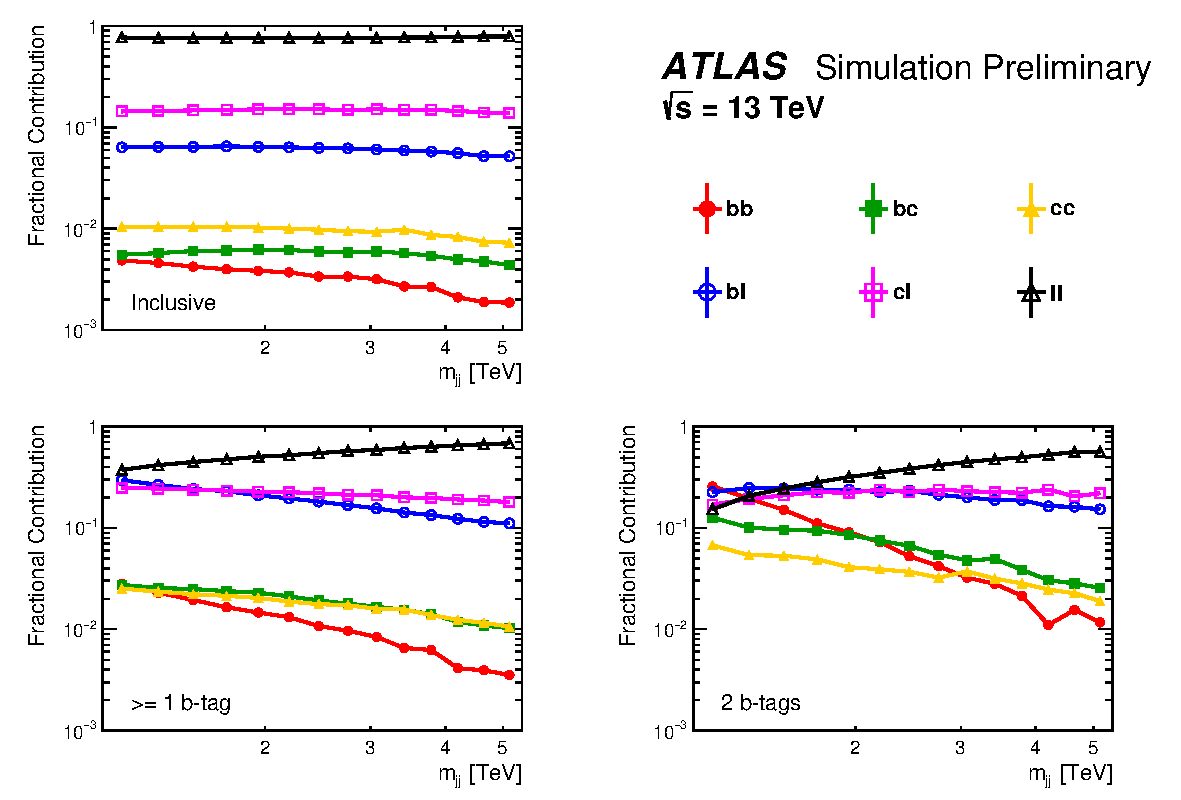
\includegraphics[width=0.88\linewidth, angle=0]{figs/Dibjet/ICHEP/evt-summer_flavcomp.pdf}
  \end{center}
  \vspace{-1.25em}
  \caption
      [The dijet flavour composition of simulated QCD dijet production as a function of dijet mass for the \summer{} data-set.]
      {The dijet flavour composition of simulated QCD dijet production as a function of dijet mass (\mjj{}) for the \summer{} data-set
        shown without applying $b$-tagging (inclusive) and for the $\geq1$ $b$-tag and 2 $b$-tag categories.
        In the legend b, c and l refer to a truth matched $b$-jet, $c$-jet and light jet respectively.
        The \summer{} data-set event selection has been applied.}
      \label{fig:evt-summer_flavcomp}
%\end{figure}
%\begin{figure}[!ht]
  \begin{center}
    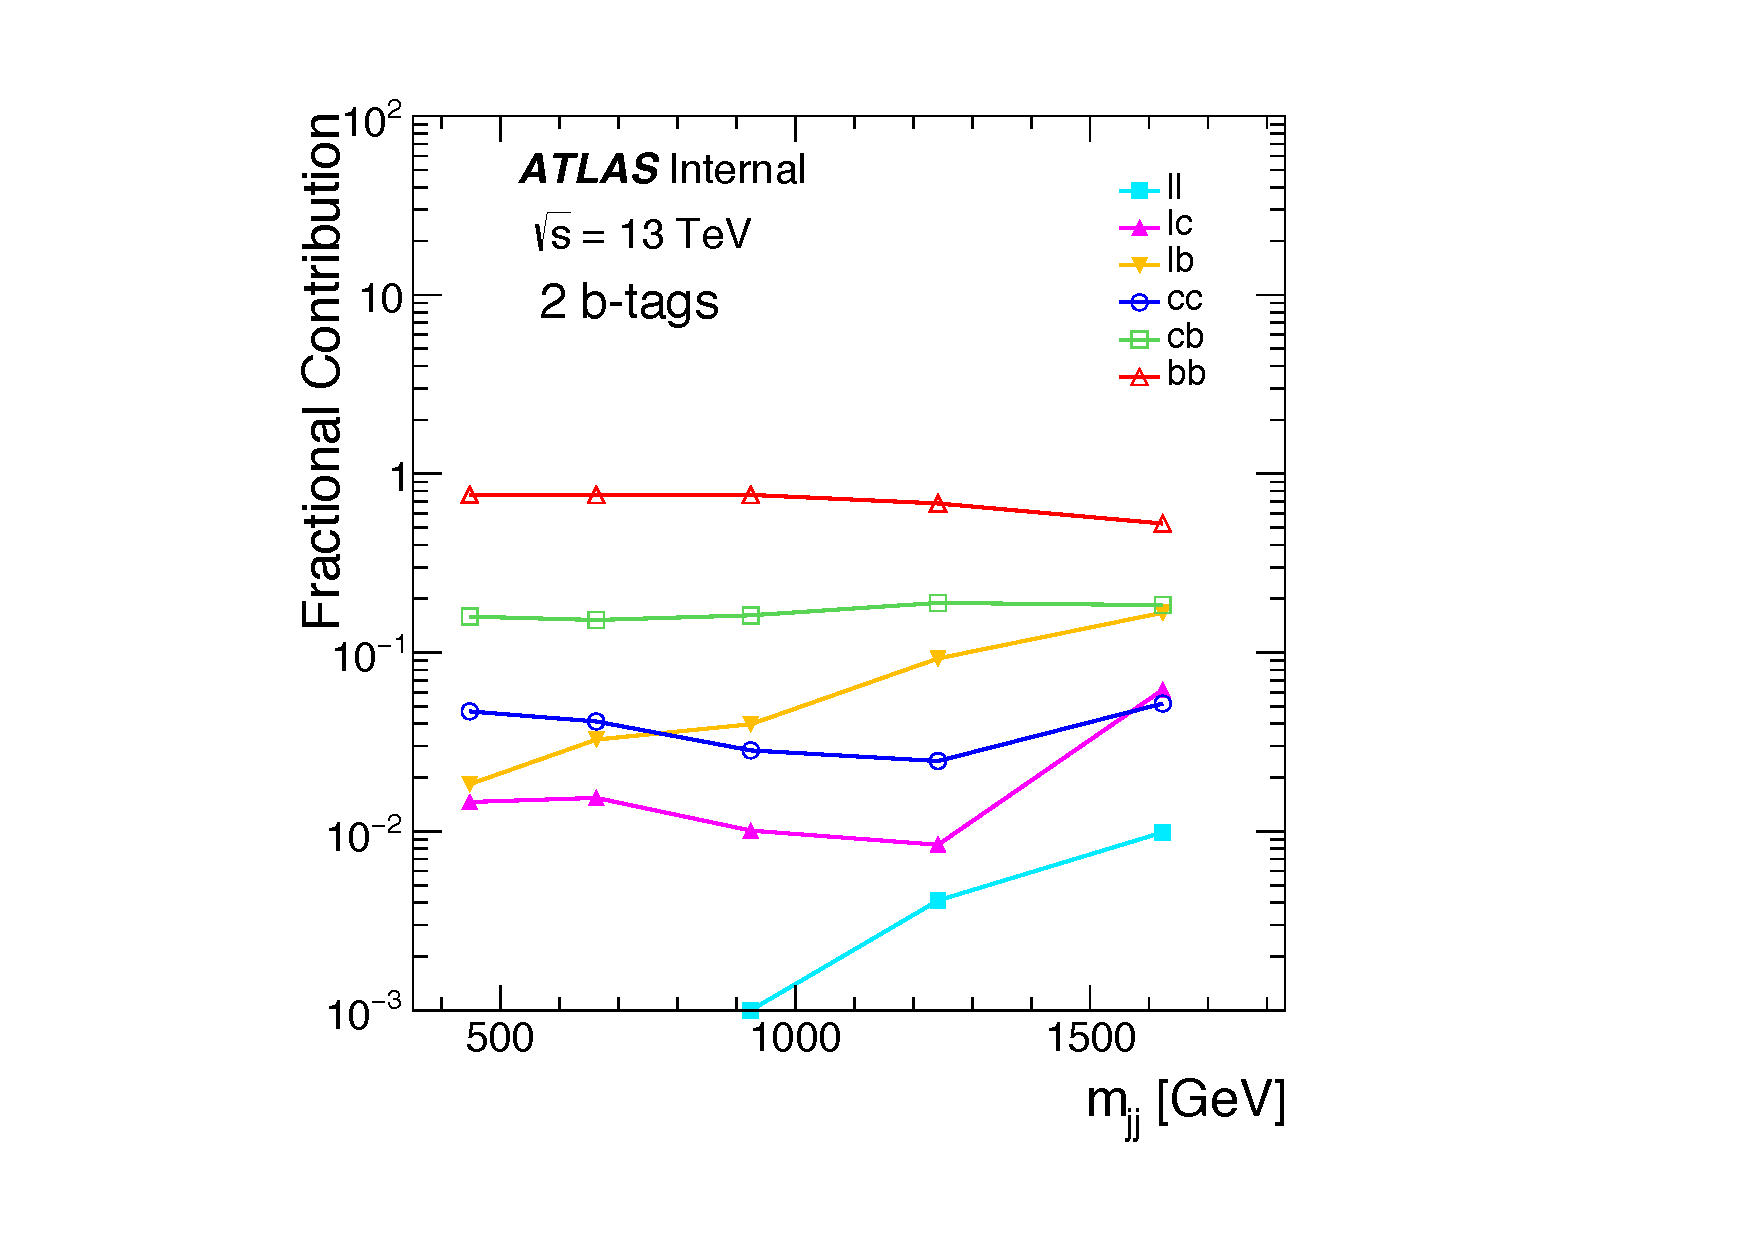
\includegraphics[width=0.43\linewidth, angle=0]{figs/Dibjet/LowMass/evt-flavcomp.pdf}
  \end{center}
  \vspace{-1.25em}
  \caption[The dijet flavour composition of simulated QCD dijet production as a function of dijet mass for the \lm{} data-set.]
          {The dijet flavour composition of simulated QCD dijet production as a function of dijet mass for the \lm{} data-set
            shown after the application of online and offline $b$-tagging requirements.
            In the legend b, c and l refer to a truth matched $b$-jet, $c$-jet and light jet respectively.
            The \lm{} data-set event selection has been applied~\cite{dibjet-full_int}.}
  \label{fig:evt-lowmass_flavcomp}
\end{figure}


\subsection{Effect of $b$-Jet Trigger Matching in the \lm{} Data-set}
\label{sec:evt-sel_btrigMatch}

As discussed in Section~\ref{sec:trig-bjet},
the double $b$-jet trigger used in the \lm{} data-set
requires that there is one online jet with \pT{}~\gt~150~GeV,
another online jet with \pT{}~\gt~50~GeV
and that both jets are $b$-tagged at the 60\% online operating point.

As described in Section~\ref{sec:evt-sel-jets}, it is required that the leading and subleading offline jet have a jet \pT{} above
200~GeV and 80~GeV respectively such that events are on the trigger plateau.
Then, in Section~\ref{sec:evt-sel-event} it was shown that in the \lm{} data-set
there is no kinematic bias in the dijet mass distribution due to the leading and subleading offline jet \pT{} cuts for \mjj{}~\gt{}~500~GeV.

However, it has been discovered that one must also consider the effect of offline jets other than the leading and subleading jet,
these jets I will refer to as `non-leading jets'.
As online and offline $b$-tagging are different processes \footnote{\ The differences are described in Section~\ref{sec:trig-bjet}.}
it is possible to have an event where the leading and subleading jet pass the online and offline jet-\pT{} requirements and are $b$-tagged offline
but one or both of the leading or subleading jets do not pass the online $b$-tagging requirements.
Such an event can still pass the double $b$-jet trigger if  a non-leading jet
passes the online jet-\pT{} requirements and is online $b$-tagged.
In this case different jets are used at the trigger level than are used in the offline analysis.
Therefore, it must be additionally shown that in the dijet mass range considered there is not a kinematic bias
due to events where a non-leading jet is used by the trigger.

A study is performed to determine the effect of the $b$-jet trigger using non-leading jets on the dijet mass spectrum.
For this study offline jets are matched to online jets in a process known as trigger matching.
An offline jet is matched to an online jet if $\Delta R$
between the jets is less than 0.4,
the matching is exclusive meaning that online jets are only matched to offline jets with the smallest $\Delta R$ separation.
%
%The matching is exclusive, which means that no online or offline jet can be involved in two matchings.
%In the case that an offline jet can be matched to two online jets, then the pair of jets with the smallest~$\Delta R$ is chosen.
%In the case where two offline jets can be matched to an online jet, the offline jet with the highest-\pT{} is chosen;
%this is done as there is a prior reason to believe that the leading and subleading offline jets are responsible
%for passing the $b$-jet trigger requirements as they are known to pass offline $b$-tagging.
%
%To keep matching exclusive the following algorithm is performed.
%Firstly, the leading offline jet is matched to the online jet with the smallest $\Delta R$, if the value of $\Delta R <$ 0.4.
%This process is repeated with the subleading offline jet, excluding online jets that have already been matched.
%The other jets are the matched in a similar manner considered in order of jet-\pT.
%

Then one can define `$b$-jet trigger matched events' as events where
the leading and subleading offline jets have successful been matched to online jets
and that these online jets pass the double $b$-jet trigger requirements described above.
In $b$-jet trigger matched events it is known that leading and subleading jet are used to pass the double $b$-jet trigger.
In events that are not $b$-jet trigger matched events, a non-leading jet has been used by the double $b$-jet trigger.

To study $b$-jet trigger matched events an additional complication has to be overcome.
To perform trigger matching the \pT, $\eta$, $\phi$ and MV2c20 output of the online jets is required.
Data from the ATLAS collaboration is processed and stored in containers known as `derivation containers'
\footnote{Formally the `derivation containers' are known as Derived Analysis Object Data (DAODs)}.
To reduce the computer resources required to analyse a derivation container
there are many types of derivation containers,
where each contains only the events and the reconstructed object information required to perform an analysis.
For the di-$b$-jet search a derivation called \textit{EXOT2} is used,
however the online jet information required for trigger matching is not present in the \textit{EXOT2} derivation containers.
Instead, a derivation container called \textit{FTAG1} is used, in which the online jet information is present.
However, in the \textit{FTAG1} derivation not all events that pass the double $b$-jet trigger are included.
Therefore, neither derivation container contains the full information required to do $b$-jet trigger matching on the full \lm{} data-set.

To overcome this problem the effect of $b$-jet trigger matching can be studied using the \textit{FTAG1} derivation
to test if there is a kinematic bias.
Firstly, one can consider the dijet mass spectrum of all events in the \textit{FTAG1} derivation
that pass the \lm{} data-set event selection before $b$-jet trigger matching is applied.
I will refer to this as the dijet mass spectrum from \textit{FTAG1}.
Figure~\ref{fig:evt-btrig_match}(a) shows the dijet mass spectrum from \textit{FTAG1}
compared to the full dijet mass spectrum from the \textit{EXOT2} derivation, where all events are present.
The full \lm{} data-set event selection has been applied to both.
The ratio shows that there is a deficit of events in the dijet mass spectrum from \textit{FTAG1} at low mass.

\begin{figure}[!ht]
  \begin{center}
    \captionsetup[subfigure]{aboveskip=0pt,justification=centering}
    \subcaptionbox{} {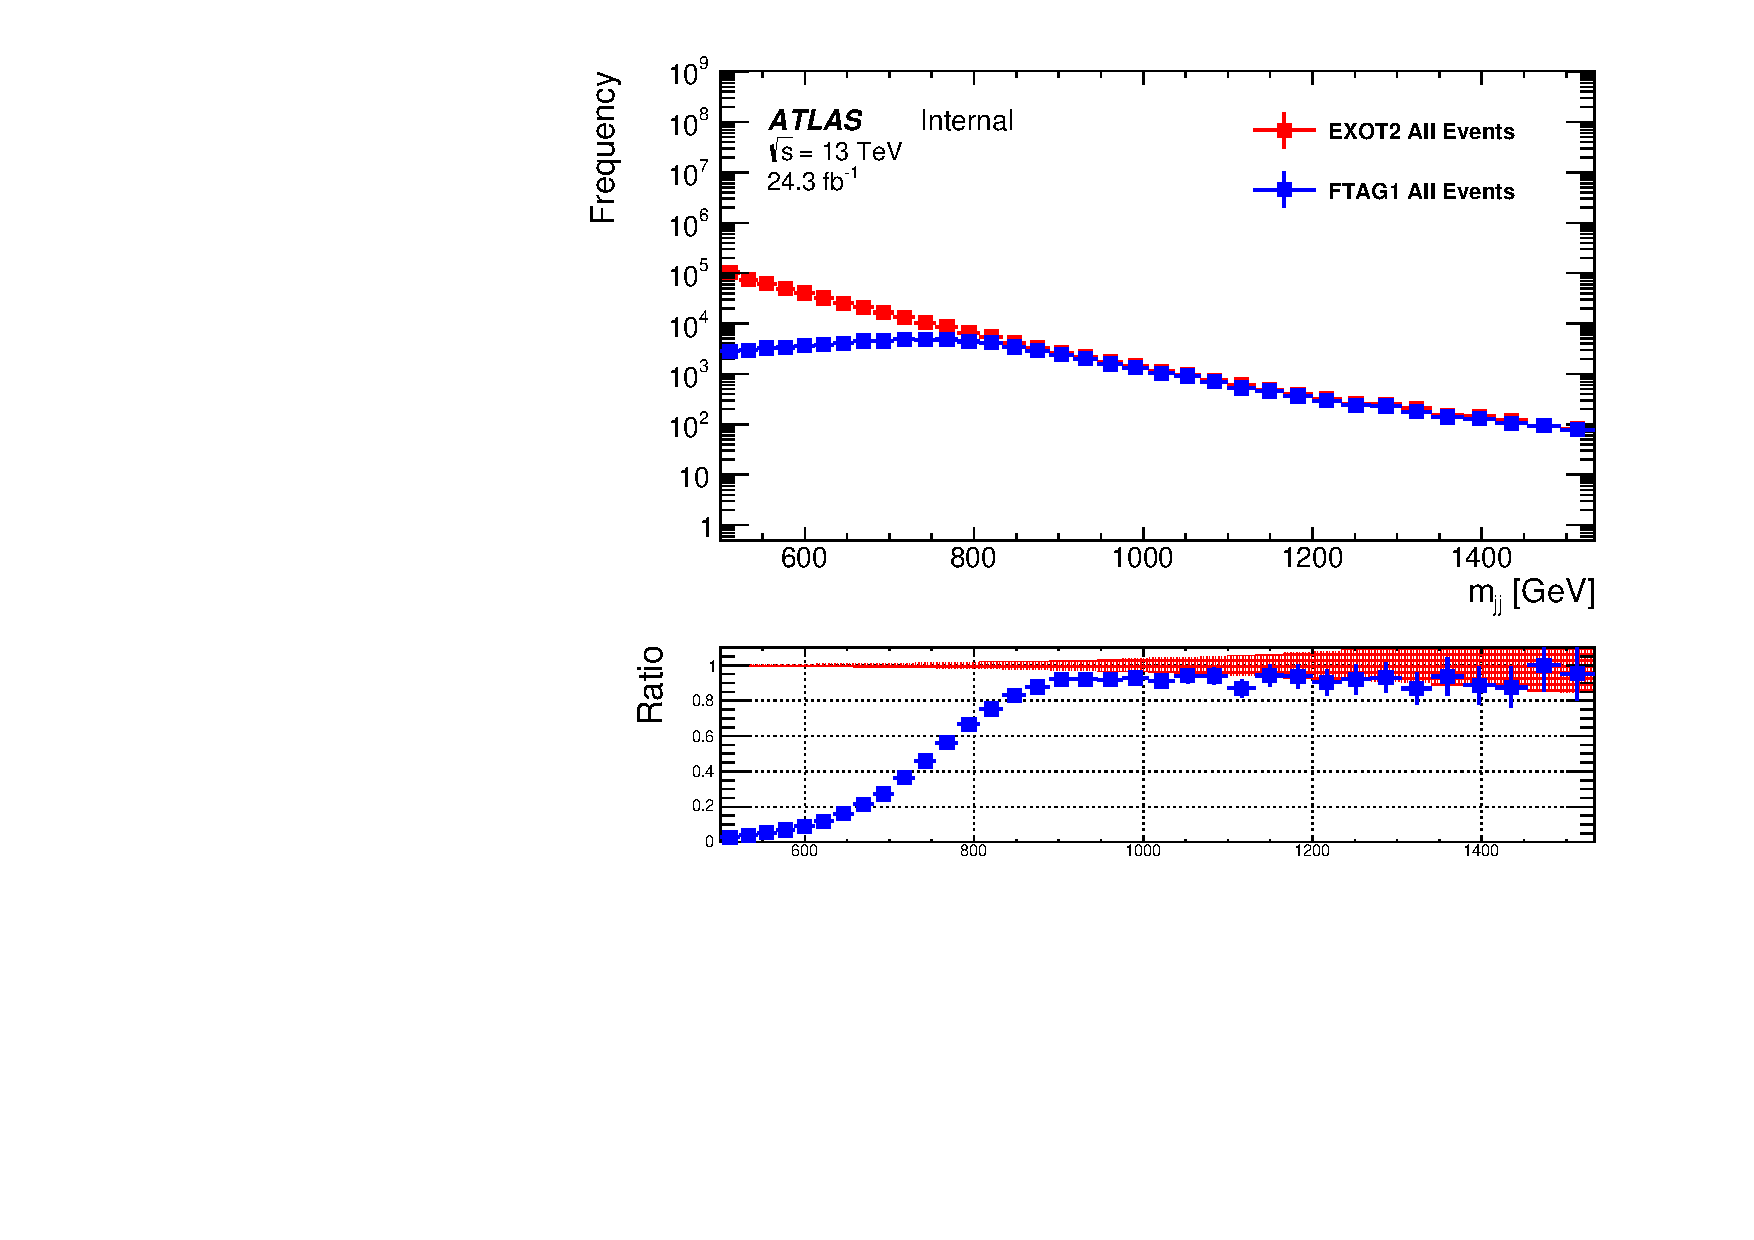
\includegraphics[width=0.5\linewidth, angle=0]{figs/Dibjet/LowMass/evt-trigmatch_exot2.pdf} }\hspace{-5mm}
    \subcaptionbox{} {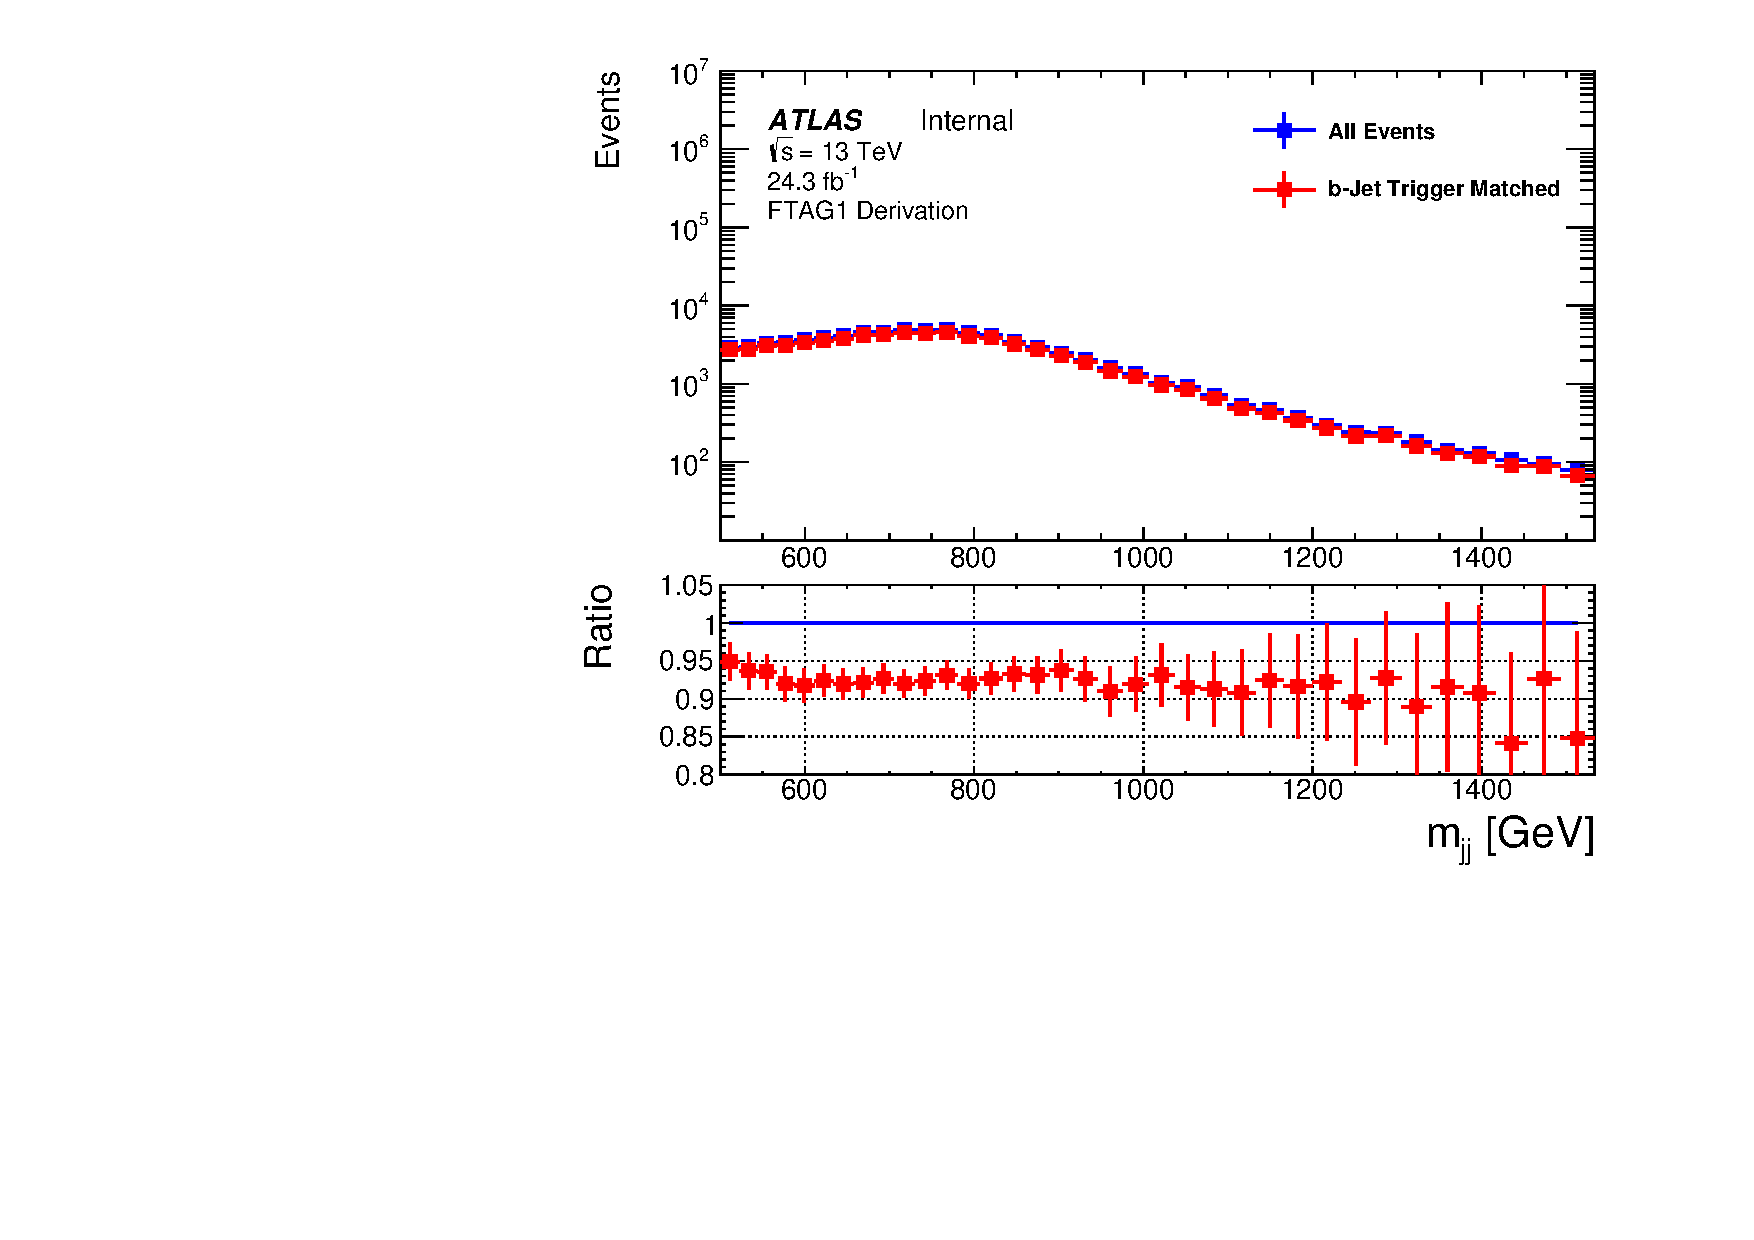
\includegraphics[width=0.5\linewidth, angle=0]{figs/Dibjet/LowMass/evt-trigmatch_ftag1.pdf} }
  \end{center}
  \vspace{-1em}
  \caption
      [A comparison of the dijet mass spectra created using the \textit{EXOT2} derivation and the \textit{FTAG1} derivation
       and a comparison of the dijet mass spectra of all events and $b$-jet trigger matched events using the \textit{FTAG1} derivation.
        For both plots the full \lm{} event selection is applied.]
      {(a) A comparison of the dijet mass (\mjj) spectra created using the \textit{EXOT2} derivation and the \textit{FTAG1} derivation.
        (b) A comparison of the dijet mass spectra of all events and $b$-jet trigger matched events using the \textit{FTAG1} derivation.
        For both plots the full \lm{} event selection is applied. Details of the derivation containers is given in the text. }
      \label{fig:evt-btrig_match}
\end{figure}

Figure~\ref{fig:evt-btrig_match}(b) shows the comparison of the dijet mass spectrum from \textit{FTAG1}
before and after the application of $b$-jet trigger matching.
The full \lm{} data-set event selection has been applied in both cases.
A ratio of the two spectra is in the lower panel.
The ratio shows that $\sim$8\% of events that
pass the \lm{} event selection do not pass $b$-jet trigger matching requirement.
In these events it can be concluded that a non-leading jet is used by the double $b$-jet trigger.
For~\mjj~\gt~566~GeV the ratio is smooth with respect to dijet mass.
However in the region 500~\lt~\mjj~\lt~566~GeV, which is shown by the first three \mjj{}~bins,
there is a clear discontinuity in the ratio plot
which indicates that there is a kinematic bias due to the double $b$-jet trigger in the final data-set.

The background estimation strategy (described in Section~\ref{sec:bkg}) requires that the dijet mass spectrum must be smooth,
therefore it is required that there is no effect that can cause a non-smooth feature in the dijet mass spectrum.
It has been shown that for~\mjj~\gt 566~GeV there is no effect from non-leading jets being used in the double $b$-jet trigger
that can cause an un-smooth feature in the final data-set.
Therefore, for the \lm{} data-set it is required that~\mjj~\gt~566~GeV.

Finally it should be noted that for future iterations of the di-$b$-jet search
the full information required for $b$-jet trigger matching will be included in the \textit{EXOT2} derivation,
and as such trigger matching can be applied such that analyses can search a dijet mass range beginning at 500~GeV.

\subsection{Event Selection Summary}
\label{sec:evt-sel-acc}

A summary of the  key components of the di-$b$-jet event selection
for each of the data-sets considered
is listed in Table~\ref{tab:evt}.

{\renewcommand{\arraystretch}{1.2}
\begin{table}[!htb]
  \begin{tabular}{|c||c|c|}
    \hline
    \textbf{Data-set}         &  \textbf{\summer{}} &  \textbf{\lm{}} \\
    \hline
    Integrated Luminosity             &       13.3 \ifb{}  &   24.3 \ifb{}         \\
    \hline
    %Trigger          & HLT\_380 & HLT\_380 & \makecell{ HLT\_j150\_bmv2c2060\_split\\\_j50\_bmv2c2060\_split} \\
    Trigger                & Single-jet       & Double $b$-jet (60\% OP) \\
    Online LJ \pT          & \gt~380~GeV      & \gt~150~GeV  \\
    Online SLJ \pT         & -                & \gt~50~GeV \\
    \hline
    Leading Jet-\pT    &  \gt~430~GeV &  \gt~200~GeV\\
    Subleading Jet-\pT &  \gt~60~GeV &  \gt~80~GeV\\
    Jet-$|\eta|$   & $<$ 2.4 & $<$ 2.0 \\
    \hline
    $\mjj$  & \gt~1378~GeV &  566 -- 1533~GeV \\
    $|y^*|$  & $<$ 0.6 & $<$ 0.6  \\
    \hline
    $b$-Tagging OP & 85\% & 70\%\\
    $b$-Tag Categories & 2 and $\geq$1 & 2 \\
\hline
\end{tabular}
\centering
\caption[A summary of the key details of the di-$b$-jet event selection applied.]
        {A summary of the key details of the di-$b$-jet event selection applied in the two data-sets considered.
          LJ refers to leading jet and SLJ refers to subleading jet.
          For full details refer to the text.}
\label{tab:evt}
\end{table}}

\newpage

To visualise events that pass the event selection,
Figure~\ref{fig:evt-vp1} show events displays for high dijet mass events that pass
the $\geq$1 and 2 $b$-tag event selection respectively.
The figure was made using the VP1 event display package~\cite{evt-vp1}.
These events pass the \summer{} data-set event selection.

\begin{figure}[!ht]
  \begin{center}
    \captionsetup[subfigure]{aboveskip=0pt,justification=centering}
      \subcaptionbox{ 2 $b$-tag \vspace{4mm}}  {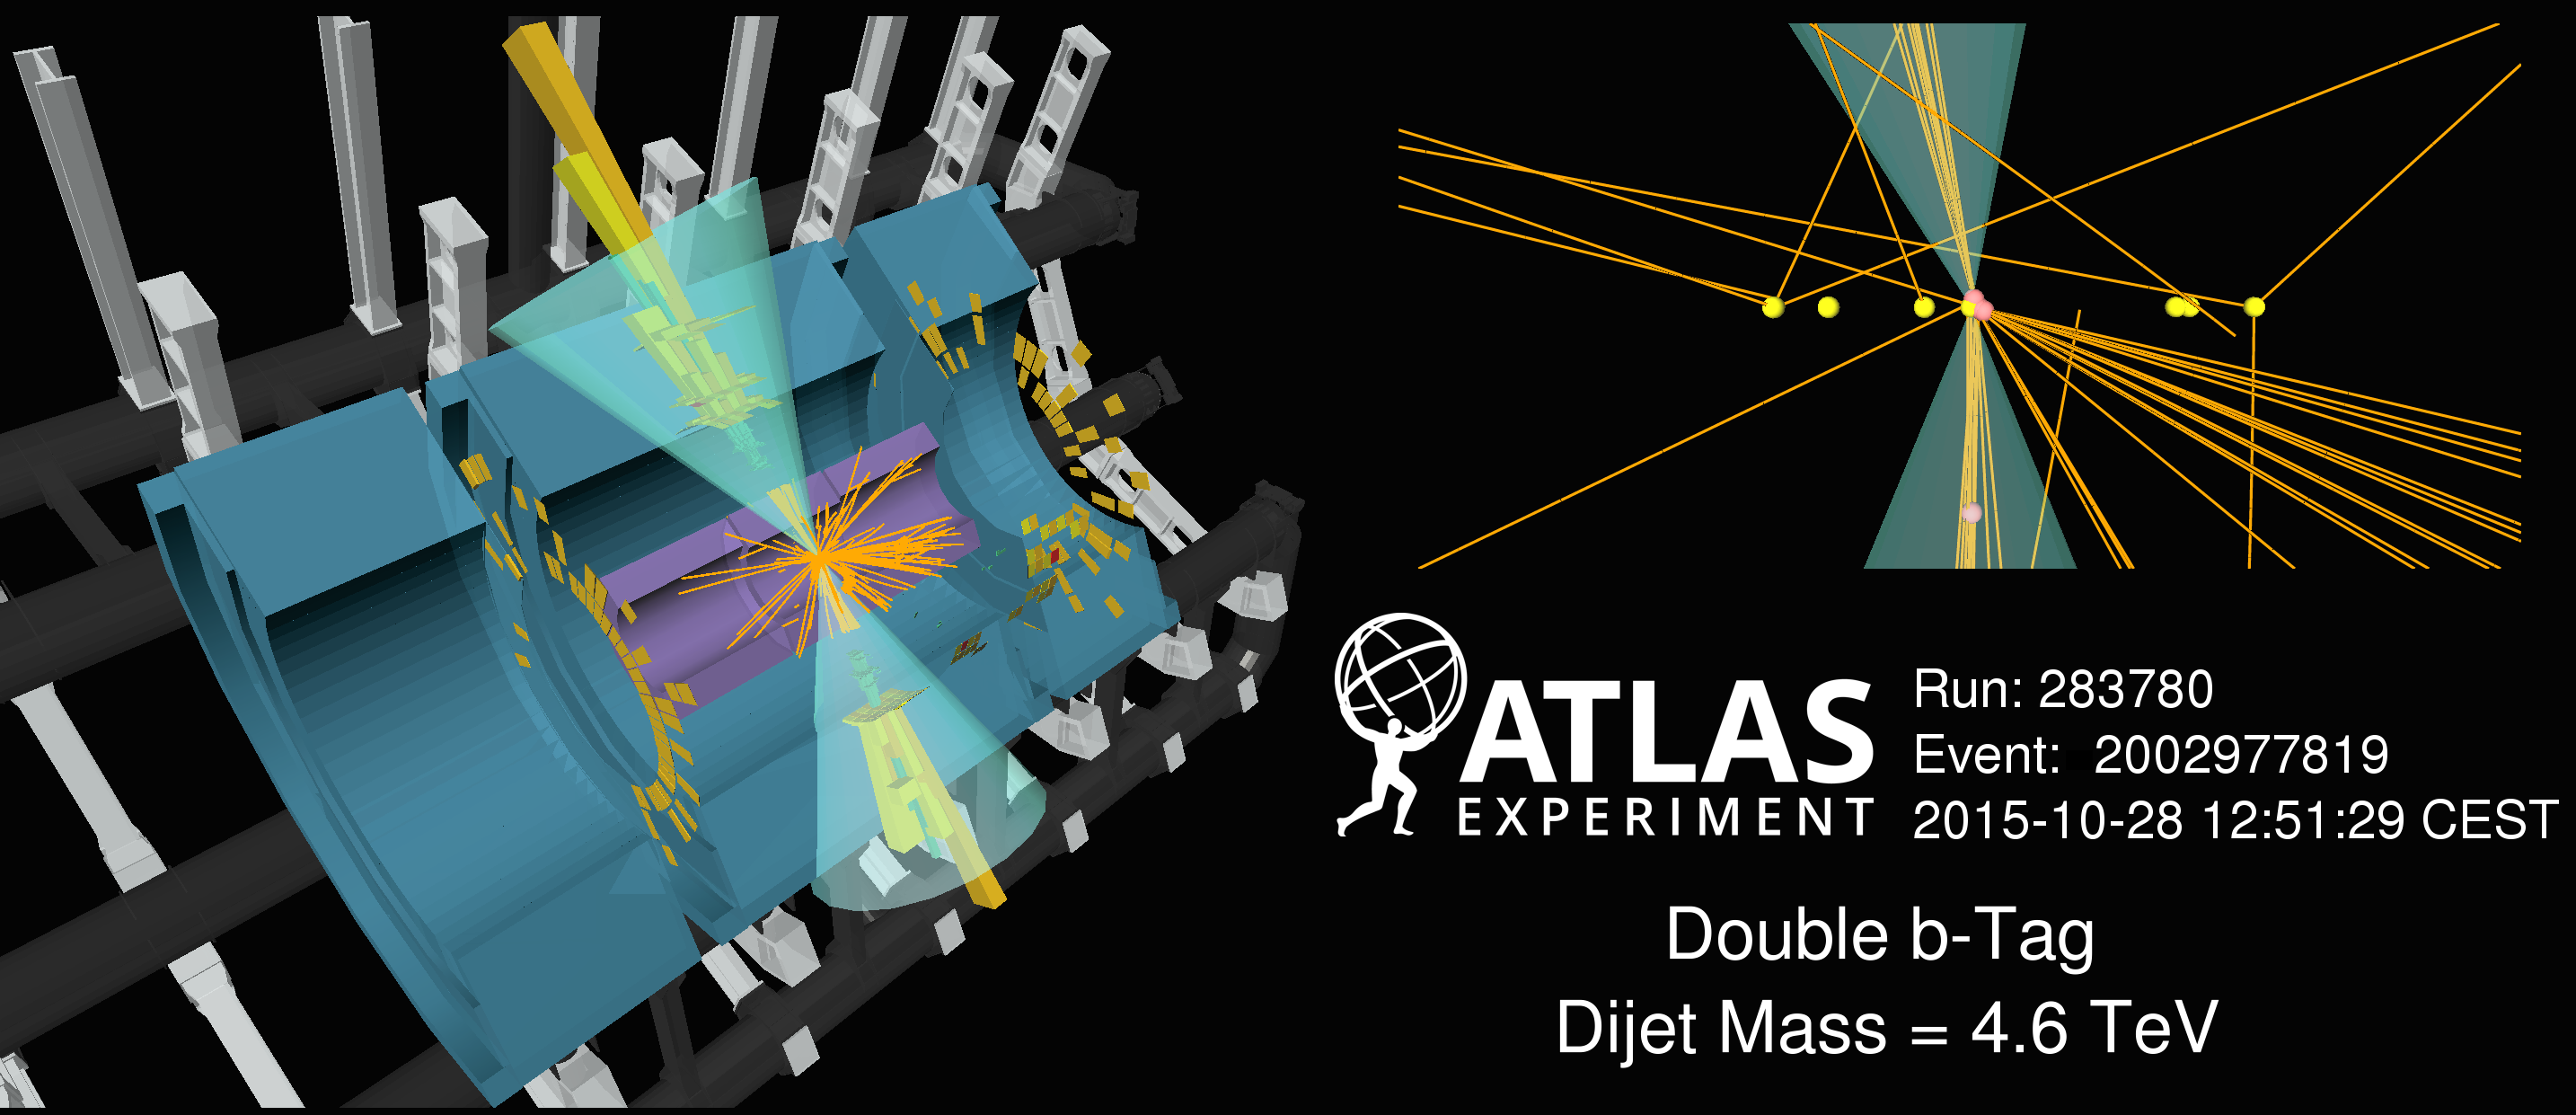
\includegraphics[width=0.99\linewidth, angle=0]{figs/Dibjet/Gen/evt-vp1_bb_edit.png}\vspace{2mm} }\\
      \subcaptionbox{ $\geq$1 $b$-tag }        {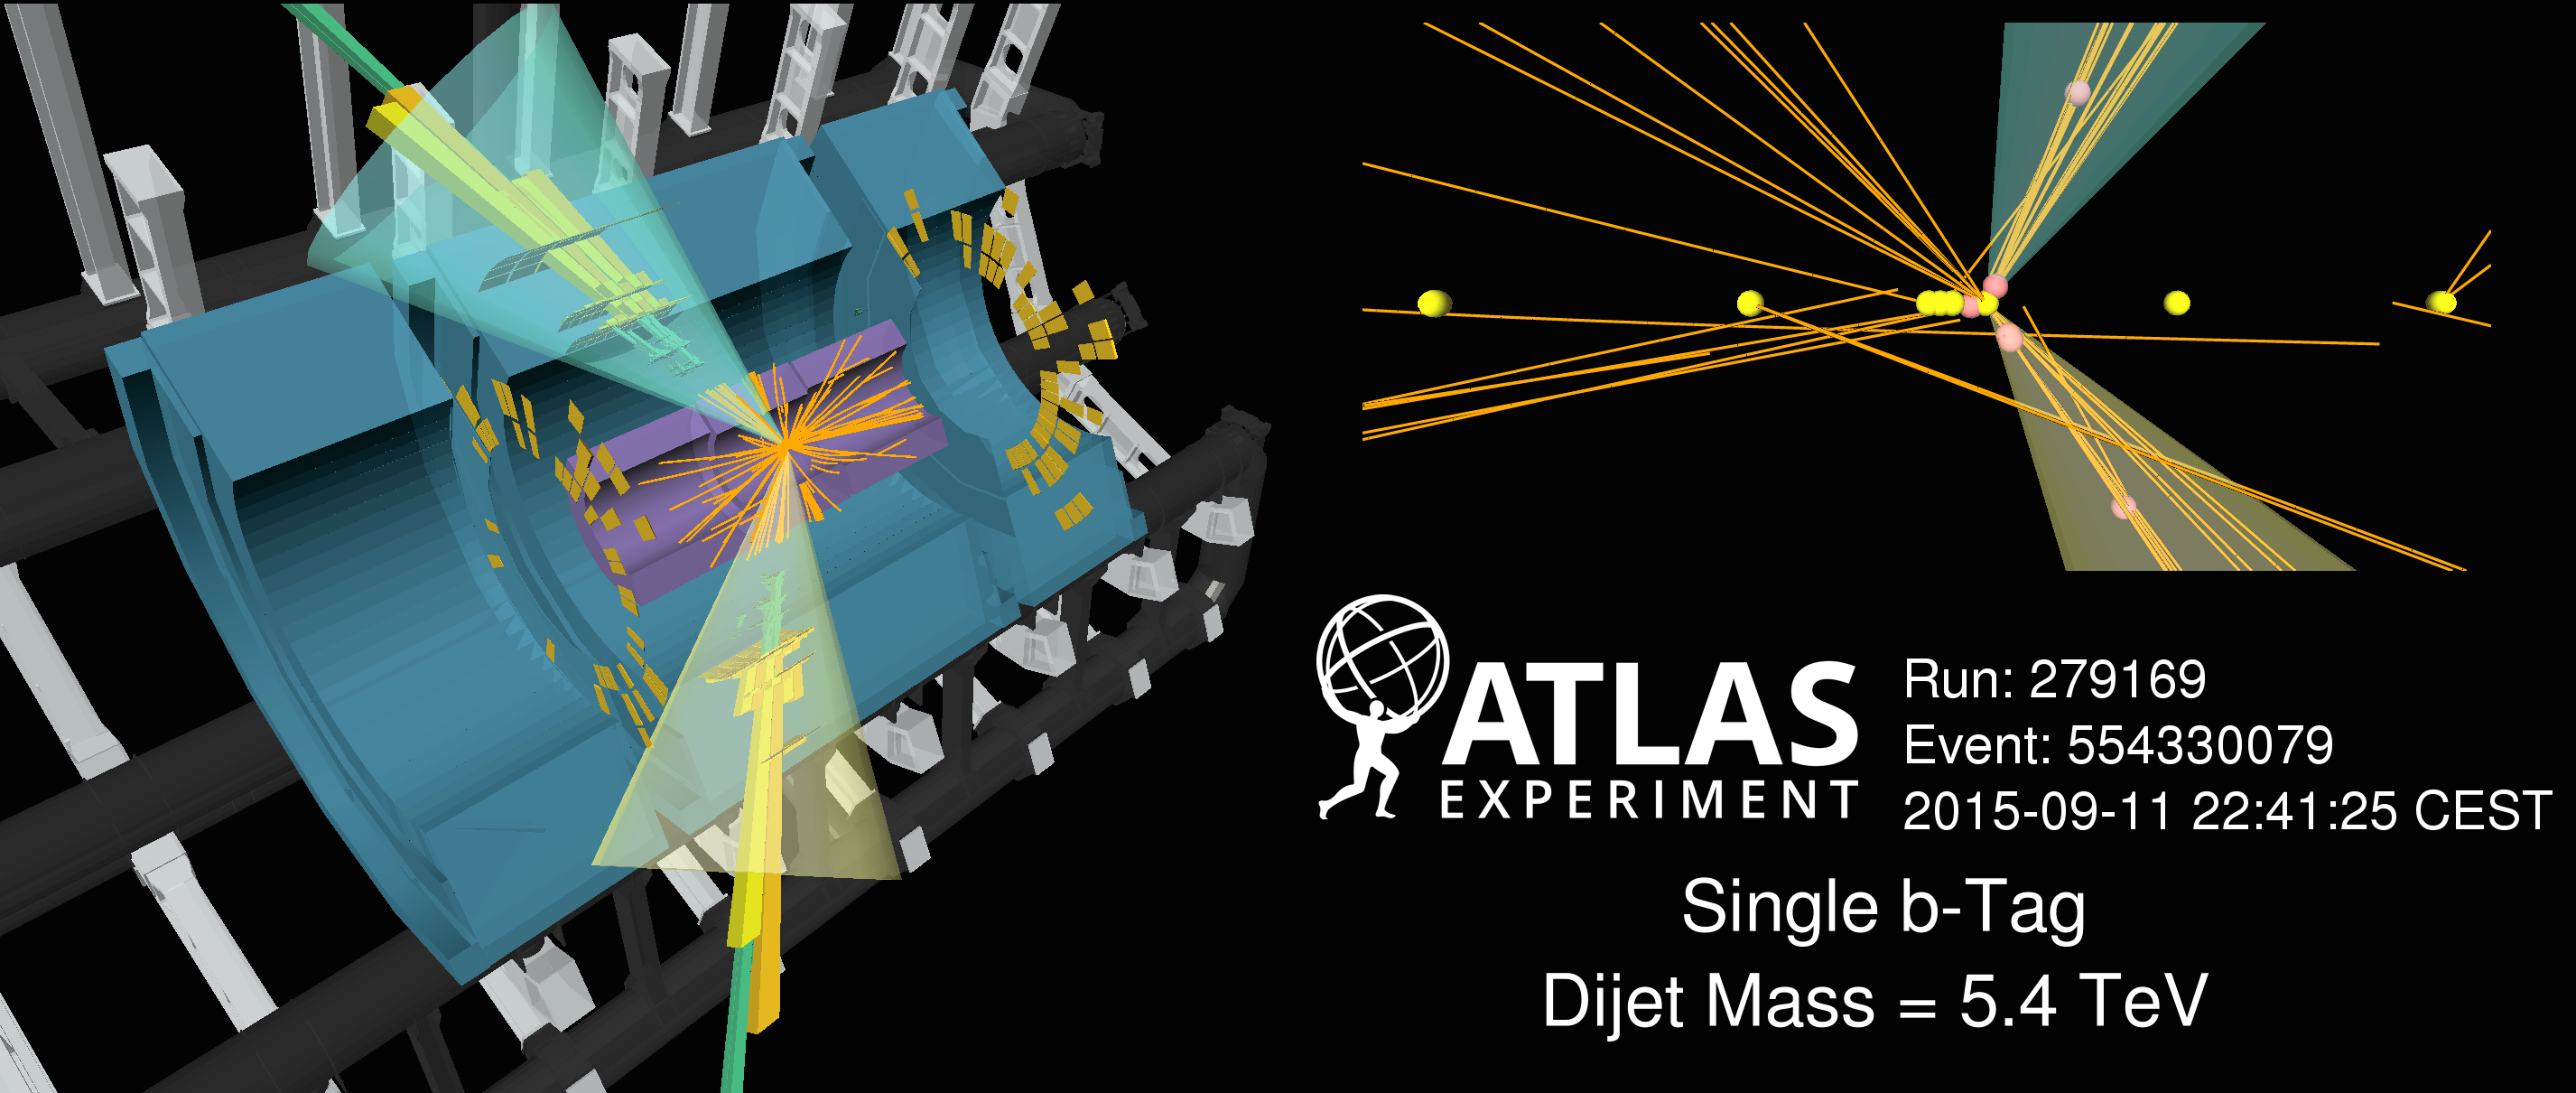
\includegraphics[width=0.99\linewidth, angle=0]{figs/Dibjet/Gen/evt-vp1_b.png}\vspace{2mm} }
  \end{center}
  \caption
      [Event displays showing high dijet mass events in the \summer{} data-set analysis.]
      {Event displays showing high dijet mass (\mjj{})~events that pass the (a) 2 and (b) $\geq$1 $b$-tag di-$b$-jet event selection in the \summer{} data-set analysis.
        The left section of the figures show a cut-away of the ATLAS detector;
        the inner detector is shown in purple, the hadronic calorimeter is shown in blue
        and the toroid magnet and supporting structure is shown in black and grey.
        The upper right section of the figures show a close-up view of the inner tracker in the $r-z$ plane.
        In both sections tracks inside the inner detector are shown in orange
        and energy deposits in the EM and hadronic calorimeter are shown in green and yellow respectively.
        The two leading jets formed are indicated by the cones, a blue cone indicates that the jet has been
        $b$-tagged and a yellow cone indicates that it has not.
        In the upper right panel the yellow spheres show the primary vertex candidates and the red spheres show the secondary vertex candidates.
      }
  \label{fig:evt-vp1}
\end{figure}

\newpage 
With the event selection now defined,
the signal acceptance of the di-$b$-jet event selection is studied
to understand the performance of the analysis selection.
The signal acceptance is also a required input to the limit setting phase of the analysis, described in Chapter~\ref{sec:lim}.
The signal acceptance multiplied by trigger efficiency is defined as the 
fraction of signal events that pass the analysis' trigger and event selection.
In addition, as $b$-tagging is a unique selection in our analysis relative to other dijet searches,
the event-tagging efficiency is also considered, which is defined as the fraction of signal events that pass
the $b$-tagging requirements given that the event has passed all other aspects of the event selection.
Signal acceptance and event tagging efficiency are estimated using the
Monte-Carlo signal templates discussed in Section~\ref{sec:evt-s+b}.

For the \summer{} data-set event selection;
Figure~\ref{fig:evt-ichep_acc}(a) shows the signal acceptance multiplied by trigger efficiency
for the $b^*$ quark and SSM $Z'$ boson signal models
as a function of the generated mass
in the case that $b$-tagging is applied and when it is not applied.
Figure~\ref{fig:evt-ichep_acc}(b) shows the event tagging efficiency
for the $b^*$ quark and SSM $Z'$ boson for a range of generated mass points
as a function of the dijet mass.
For the SSM $Z'$ boson only decays to $b$-quarks are considered.
In both plots the $b$-tagging category used is labelled in the legend.

\begin{figure}[!ht]
  \begin{center}
    \captionsetup[subfigure]{aboveskip=0pt,justification=centering}
    \subcaptionbox{Signal acceptance multiplied \\by trigger efficiency}{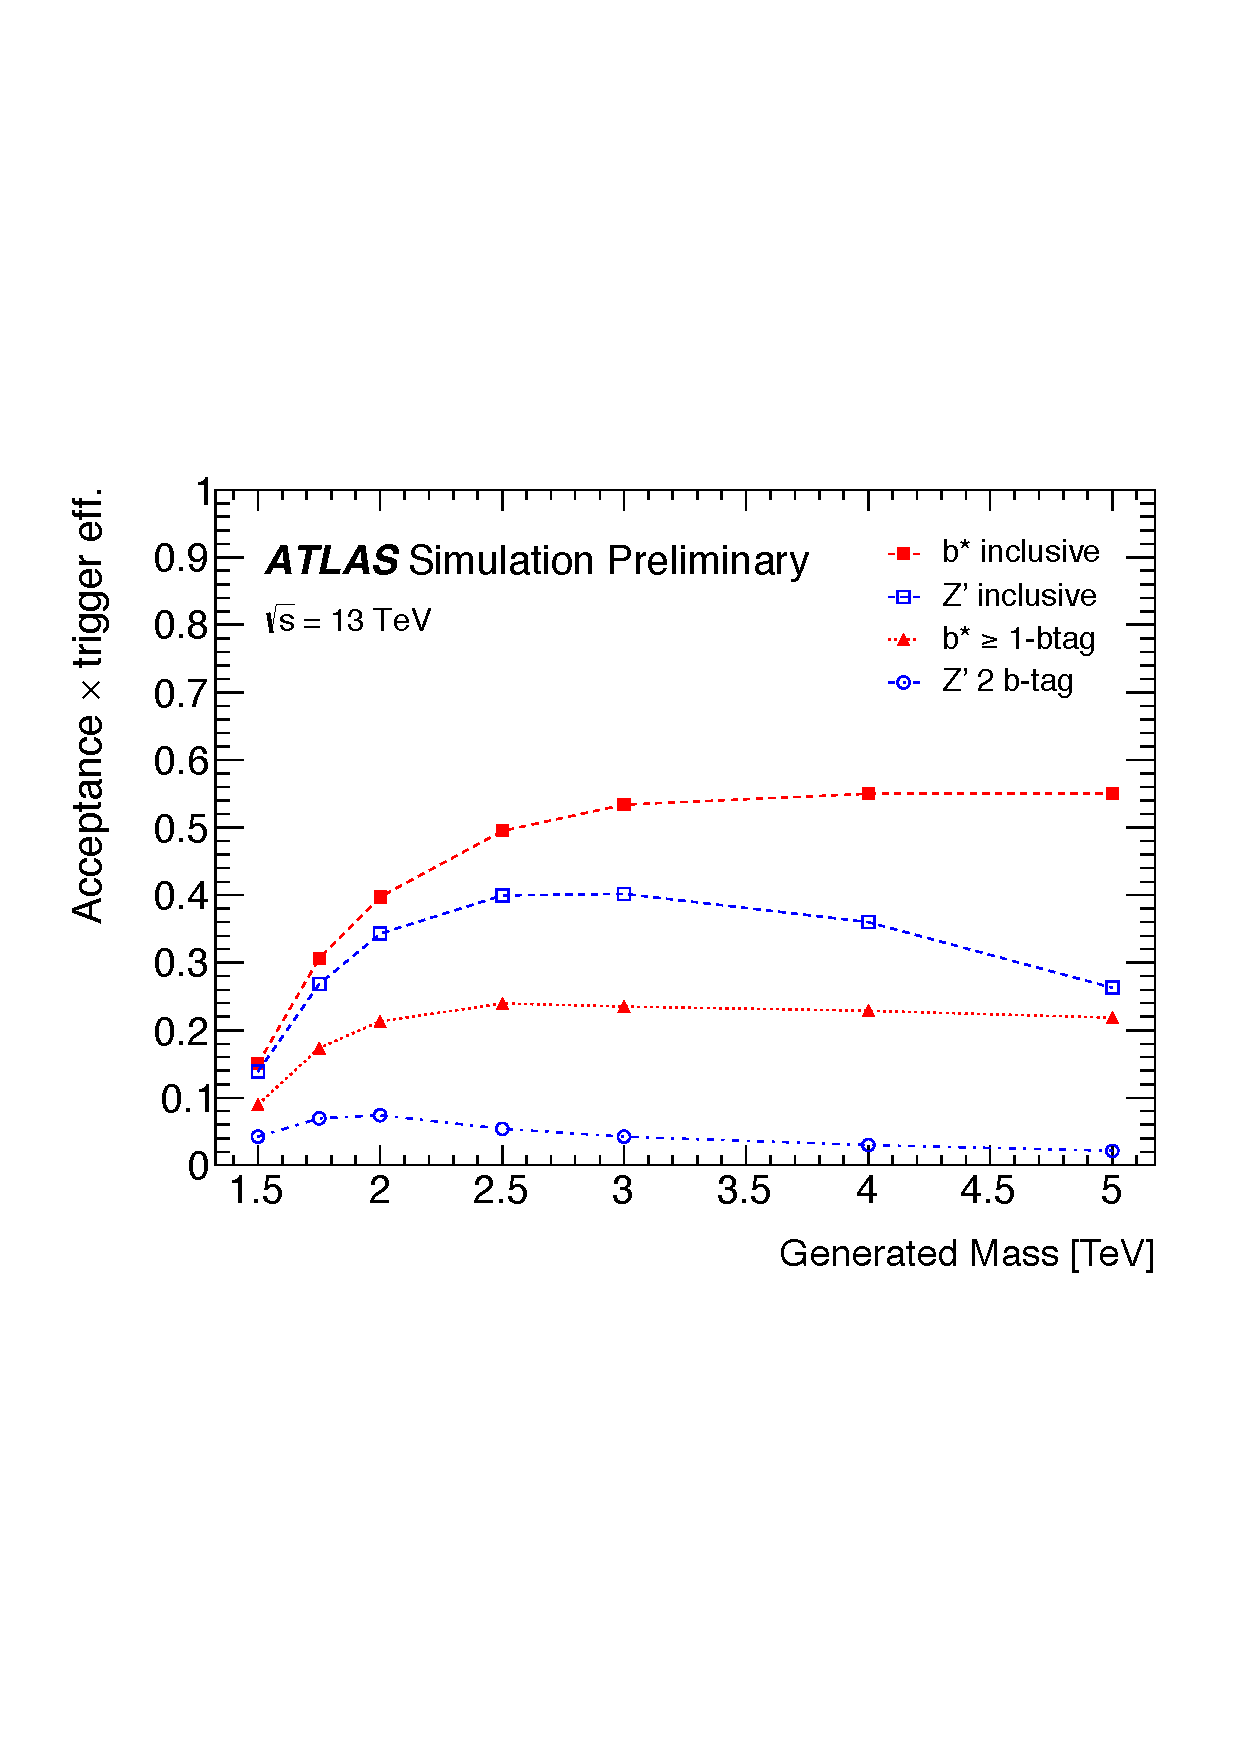
\includegraphics[width=0.48\linewidth, angle=0]{figs/Dibjet/ICHEP/evt-acc_generated.pdf} }
    \subcaptionbox{Event tagging efficiency}{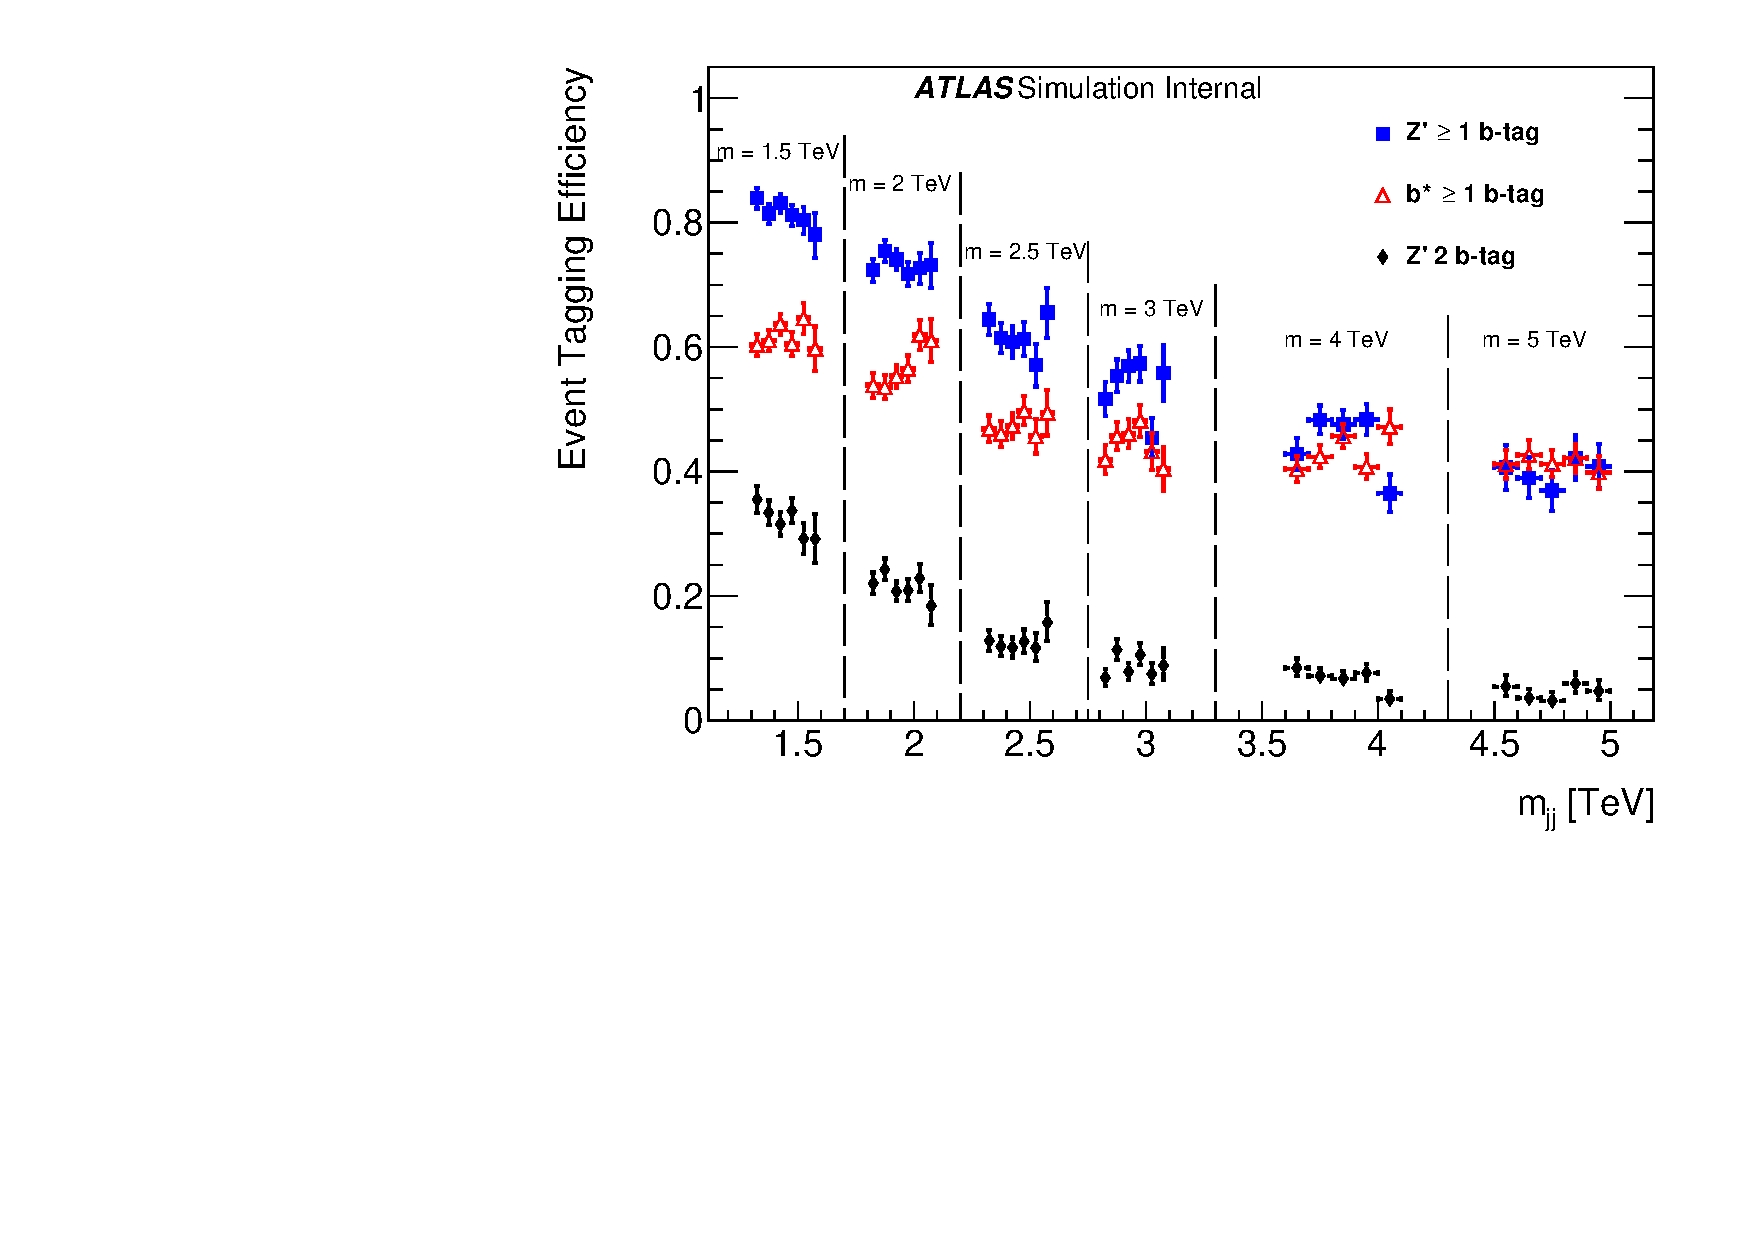
\includegraphics[width=0.49\linewidth, angle=0]{figs/Dibjet/ICHEP/evt-tagEff.pdf} }
  \end{center}
  \vspace{-1em}
  \caption[Plots to show the acceptance of the \summer{} data-set event selection for the $b^*$ quark and SSM $Z'$ boson signal models.]
          {Plots to show the acceptance of the \summer{} data-set event selection for the $b^*$ quark and SSM $Z'$ boson signal models.
            Panel (a) shows the signal acceptance multiplied by trigger efficiency as a
            function of the generated mass of the signal model, in the case where $b$-tagging has been applied and not.
            Panel (b) shows the event tagging efficiency as a function of the dijet mass (\mjj{})
            for a range of generated masses, $m$, as indicated on the plot.
            In both figures the $b$-tagging categories used are indicated in the legend.
            %Details of the \summer{} data-set event selection are described in the text.
            Figures taken from~\cite{dibjet-ichep_conf}.} 
  \label{fig:evt-ichep_acc}
\end{figure}

%For the \hm{} data-set event selection;
%Figure~\ref{fig:evt-hm_acc}(a) shows the signal acceptance multiplied by trigger efficiency
%for the $b^*$ quark, SSM $Z'$ boson and Dark Matter mediator (DM) $Z'$ boson signal models
%as a function of the generated mass.
%For both models the signal acceptance is shown before and after the
%dijet mass and $b$-tagging requirements are applied.
%Figure~\ref{fig:evt-hm_acc}(b) shows the event tagging efficiency
%for the $b^*$ quark and SSM $Z'$ boson for a range of generated mass points
%as a function of the dijet mass (\mjj{}).
%The SSM $Z'$ boson is used to show the event tagging efficiency such that the
%comparisons can be made between the different data-sets.
%In both plots the $b$-tagging category used is labelled in the legend.
%
%\begin{figure}[!ht]
%  \begin{center}
%    \captionsetup[subfigure]{aboveskip=0pt,justification=centering}
%    \subcaptionbox{Signal acceptance multiplied \\by trigger efficiency}{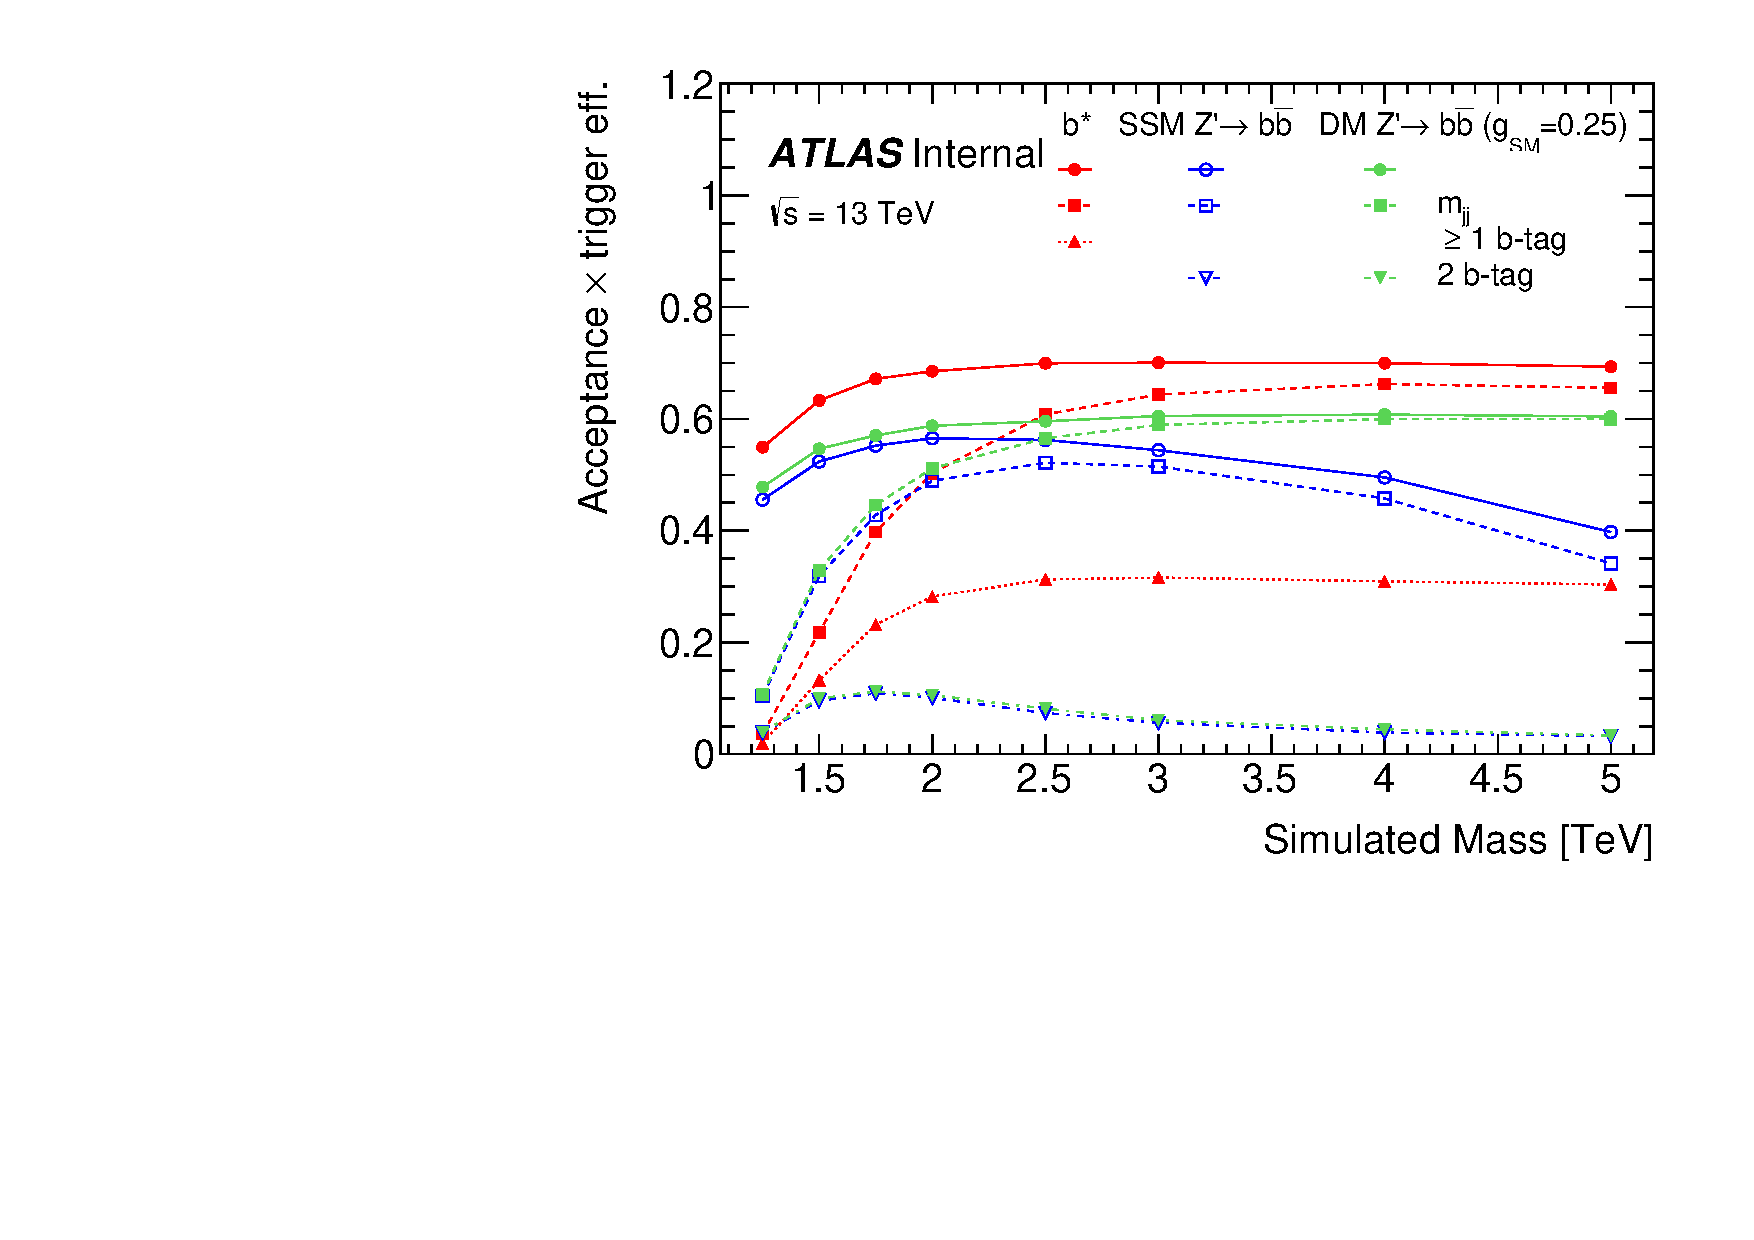
\includegraphics[width=0.48\linewidth, angle=0]{figs/Dibjet/HighMass/evt-acc.pdf} }
%    \subcaptionbox{Event tagging efficiency}{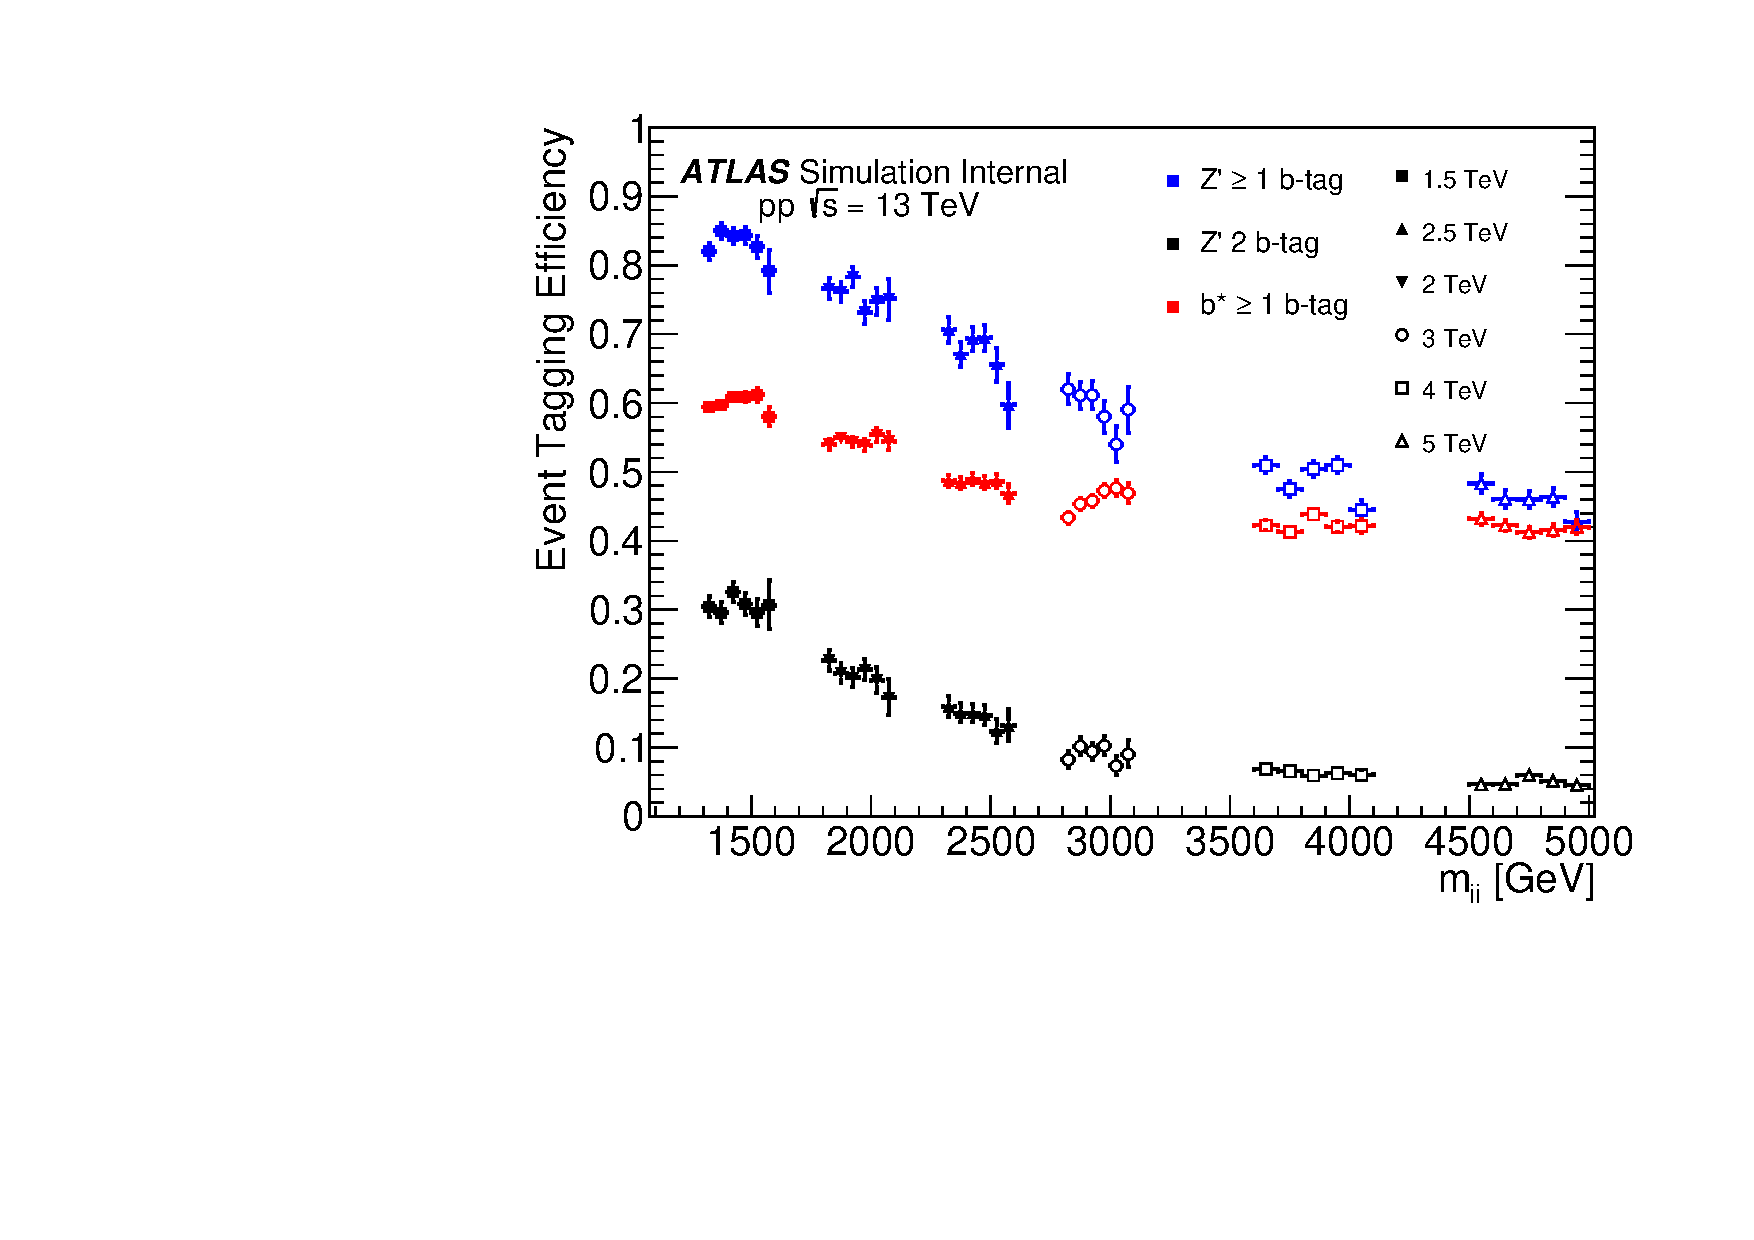
\includegraphics[width=0.49\linewidth, angle=0]{figs/Dibjet/HighMass/evt-tagEff.pdf} }
%  \end{center}
%  \caption[Plots to show the acceptance of the \hm{} data-set event selection for the $b^*$ quark,
%            Sequential Standard Model (SSM) $Z'$ boson and Dark Matter mediator (DM) $Z'$ boson signal models.
%            Panel (a) shows the signal acceptance multiplied by trigger efficiency as a
%            function of the generated mass of the signal model, before and after the
%            dijet mass and $b$-tagging requirements are applied.
%            Panel (b) shows the event tagging efficiency as a function of the dijet mass (\mjj{}),
%            for the $b^*$ quark and SSM $Z'$ boson models
%            for a range of generated masses, $m$, as indicated in the legend.
%            In both figures the $b$-tagging categories used are indicated in the legend.
%            Details of the \hm{} data-set event selection are described in the text.]
%          {Plots to show the acceptance of the \hm{} data-set event selection for the $b^*$ quark,
%            Sequential Standard Model (SSM) $Z'$ boson and Dark Matter mediator (DM) $Z'$ boson signal models.
%            Panel (a) shows the signal acceptance multiplied by trigger efficiency as a
%            function of the generated mass of the signal model, before and after the
%            dijet mass and $b$-tagging requirements are applied.
%            Panel (b) shows the event tagging efficiency as a function of the dijet mass (\mjj{}),
%            for the $b^*$ quark and SSM $Z'$ boson models
%            for a range of generated masses, $m$, as indicated in the legend.
%            In both figures the $b$-tagging categories used are indicated in the legend.
%            Details of the \hm{} data-set event selection are described in the text.
%            Figures taken from~\cite{dibjet-full_int}.} 
%  \label{fig:evt-hm_acc}
%\end{figure}

For the \lm{} data-set event selection;
Figure~\ref{fig:evt-lm_acc}(a) shows the signal acceptance multiplied by trigger efficiency
for the SSM $Z'$ boson and  Dark Matter inspired (DM) $Z'$ boson signal models as a function of the generated mass.
For both models the signal acceptance is shown before and after the
dijet mass and offline $b$-tagging requirements are applied.
The signal acceptance is considerably lower for the DM $Z'$ boson model in the \lm{} data-set
as decays to light, $c$ and $b$ quarks are considered
whilst for the SSM model only decays to $b$-quarks are considered.
Figure~\ref{fig:evt-lm_acc}(b) shows the event tagging efficiency
of just online $b$-tagging and the combination of online and offline $b$-tagging
for the SSM $Z'$ boson for a range of generated mass points
as a function of the dijet mass,~\mjj.

\begin{figure}[!htb]
  \begin{center}
    \captionsetup[subfigure]{aboveskip=0pt,justification=centering}
    \subcaptionbox{Signal acceptance multiplied \\by trigger efficiency}{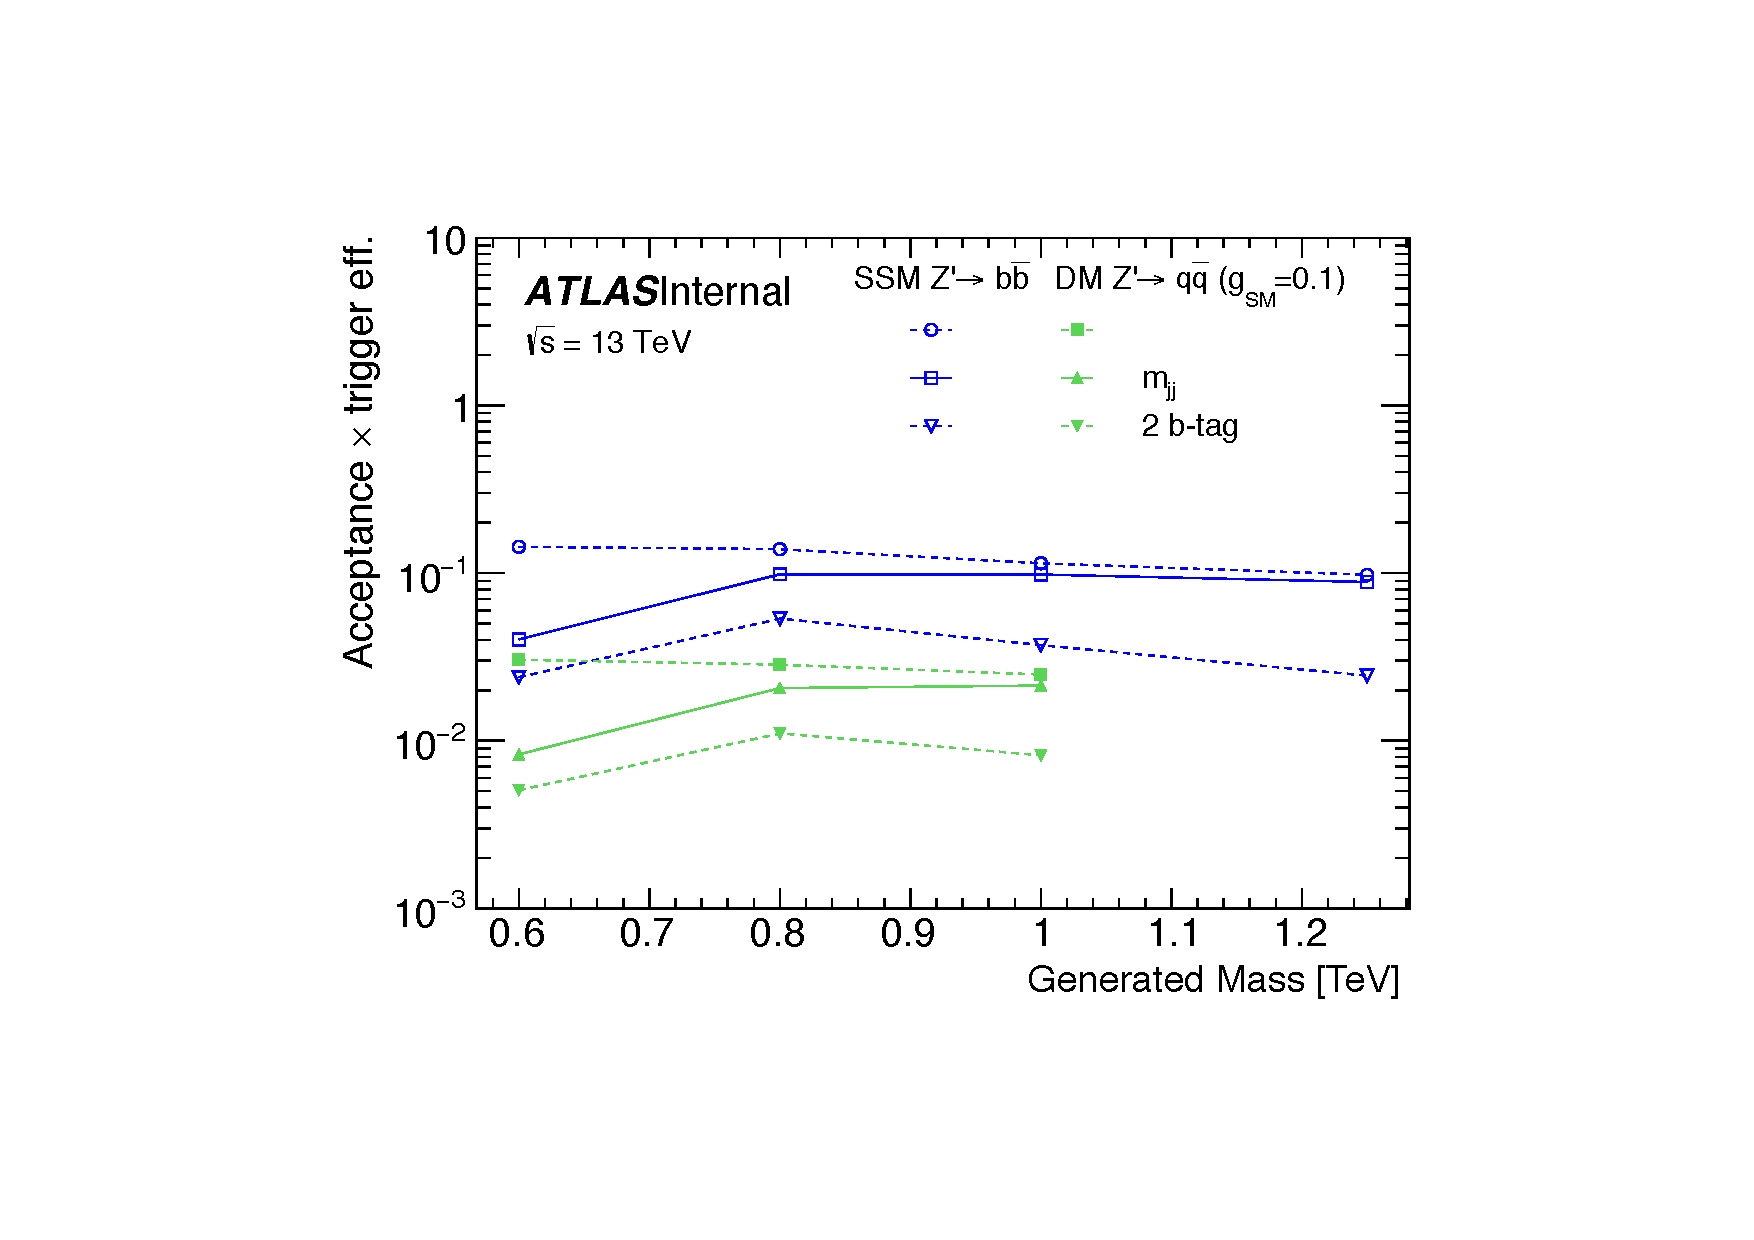
\includegraphics[width=0.49\linewidth, angle=0]{figs/Dibjet/LowMass/evt-acc_generated.pdf} }
    \subcaptionbox{Event tagging efficiency}{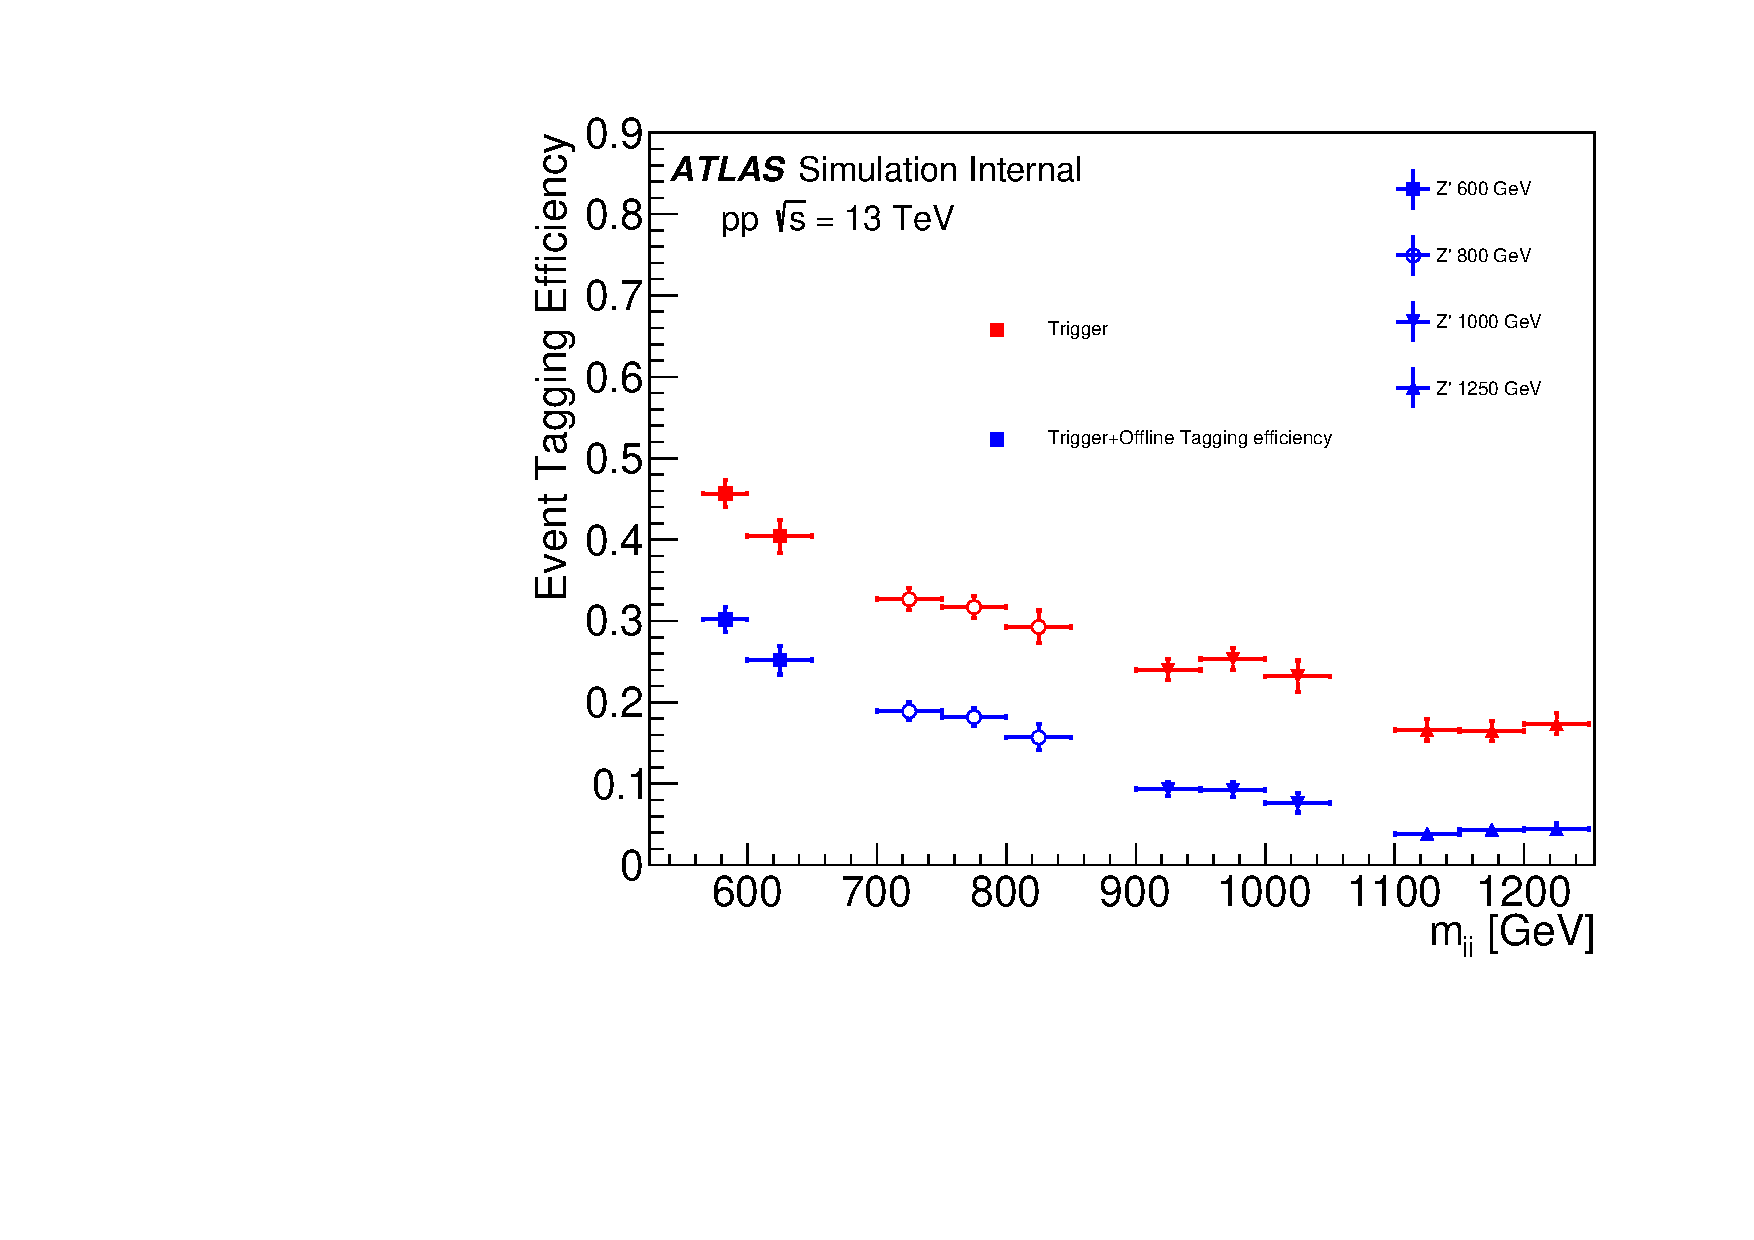
\includegraphics[width=0.48\linewidth, angle=0]{figs/Dibjet/LowMass/evt-tagEff.pdf} }
  \end{center}
  \vspace{-1em}
  \caption[Plots to show the acceptance of the \lm{} data-set event selection for the
    Sequential Standard Model (SSM) $Z'$ boson and Dark Matter inspired (DM) $Z'$ boson signal models.]
          {Plots to show the acceptance of the \lm{} data-set event selection for the
            Sequential Standard Model (SSM) $Z'$ boson and Dark Matter inspired (DM) $Z'$ boson signal models.
            Panel (a) shows the signal acceptance multiplied by trigger efficiency as a
            function of the generated mass of the signal model, before and after the
            dijet mass and offline $b$-tagging requirements are applied.
            Panel (b) shows the event tagging efficiency of just online $b$-tagging and the combination of online and offline $b$-tagging
            as a function of the dijet mass,~\mjj, for the SSM $Z'$ boson 
            at a range of generated masses, $m$, as indicated in the legend.
            %Details of the \lm{} data-set event selection are described in the text.
            Figures taken from~\cite{dibjet-full_int}.} 
  \label{fig:evt-lm_acc}
\end{figure}

There are a few features of the signal acceptance and tagging efficiency that should be commented on.
There is a reduced signal acceptance at lower generated masses
due to the dijet mass requirement of the event selection. 
%because the dijet mass template 
%has a bias towards low mass events which
%can be rejected by the dijet mass requirements of the event selection.
%The low mass bias is caused by a preference for low values of dijet mass by the PDFs.
In addition, the event tagging efficiency decreases at high values of dijet mass
due to a lower performance of $b$-tagging at high jet-\pT,
which has been discussed in Section~\ref{sec:obj-bjets_MV2}.
Finally, in Figure~\ref{fig:evt-ichep_acc} the $b^*$ quark has a similar tagging efficiency
as the $Z'$ boson in the $\geq$1 $b$-tag category when~\mjj~\gt~3 TeV;
whilst naively one would expect that the SSM $Z'$ boson should have a higher
event tagging efficiency as it decays to two $b$-quarks,
the gluon from the $b^*$ quark decay can split into a pair of lower \pT{} $b$-quarks
which can often be $b$-tagged leading to a similar event tagging efficiency.

